\chapter{Výběr a návrh elektroniky}
Výběr elektronických součástek probíhal dle jejich parametrů, využití, dostupnosti a~ceny. Nejdříve byla vybrána bezdrátová technologie a mikrokontrolér a v~závislosti 
na tom vše ostatní. 

Celkový návrh obsahuje výběr senzorů doteku, zvukových a vizuálních signalizací a případných potřebných převodníků. 

\section{Bezdrátová technologie}
Ke komunikaci Univerzálních modulů mezi sebou byla zvolena technologie LoRa a~pro bezdrátovou konfiguraci Univerzálních modulů byla zvolena technologie WiFi. 

\subsection{WiFi}
Pro bezdrátovou konfiguraci byla vybrána WiFi technologie, protože ji má k~dispozici každý ve svém telefonu a notebooku. Zároveň ji každý laik umí základně ovládát. Jedná se 
o~rozšířenou technologii. 
Propojení bude tedy jednoduché a nastavování her může probíhat na webové stránce, kde bude seznam módů, ve kterých umí Univerzální modul pracovat. U~jednotlivých her se poté 
budou moci nastavovat 
další parametry. Po nastavení se konfigurace pošle právě pomocí WiFi do Univerzálního modulu. Některé mikrokontroléry mají WiFi zabudovanou, takže jedním z~kritérií pro výběr 
mikrokontroléru se stala právě WiFi, která musí být jeho součástí. 

\subsection{LoRa}
Tato technologie byla zvolena především pro možnost rozšíření využití Univerzálního modulu. Pro toto využití byla vybrána technologie LoRa především kvůli komunikačnímu dosahu. 
Může být využita pro komunikaci Univerzálních modulů mezi sebou. Jednotlivé Univerzální moduly si tak mohou předávat informace například o~aktuálně svítící barvě nebo
o~stisknutých tlačítkách. Využití je
závislé na konkrétní aktivitě. U~některých her může být například žádoucí, aby po přepínání nesvítily všechny Univerzální moduly stejnou barvou a díky této komunikaci bude moci 
být takovým stavům zabráněno. Jedná se sice o~dražší technologii, 
ale ne na tolik, aby ji nebylo možné v~tomto zařízení použít. Outdoorové aktivity se většinou odehrávají na prostranství, která mají velkou rozlohu. LoRa je jedinou
dostupnou technologií, která na velké vzdálenosti spolehlivě komunikuje.  

Byl vybrán bezdrátový LoRa modul E22-900T22D od firmy EBYTE. Tento modul komunikuje s~mikrokontrolérem pomocí UART sběrnice \cite{LoRa_ebyte}. Jeho napájecí napětí je od 
2,1 V~do 5,5 V~a komunikační napětí je 3,3 V~\cite{LoRa_ebyte}. Rozsah komunikačních frekvencí bezdrátového modulu E22-900T22D je 850,125 MHz až 930,125 MHz a~ve výchozím 
stavu je nastavena na 868,125 MHz \cite{LoRa_ebyte}. Toto je frekvence, na které je v~ČR povoleno komunikovat a to s~maximálním vyzařovaným výkonem 25 mW \cite{CTU}. 
Maximální povolený pracovní cyklus je 1 \% \cite{CTU}. %pracovní cyklus = max duty cycle 
V~běžném režimu je spotřeba přibližně 151 mA a v~režimu spánku 2 $\mu$A \cite{LoRa_ebyte}. Tento bezdrátový modul má externě připojitelnou anténu typu SMA-K s~50 $\Omega$ 
impedancí \cite{LoRa_ebyte}.

LoRa modul E22-900T22D je připojen k~mikrokontroléru pomocí komunikačních pinů RX a TX sběrnice UART. Napájecí napětí tohoto modulu je spínáno mikrokontrolérem, aby jej 
šlo v~případě nízkého napětí baterie odpojit. Pin AUX slouží k~indikaci funkčního stavu modulu. Při specifických aplikacích slouží pro probuzení externího mikrokontroléru. 
Pomocí pinů M0 a M1 lze přepínat bezdrátový modul do různých režimů. Pokud jsou oba piny v~logické 1, 
tak je modul přepnut do režimu spánku \cite{LoRa_ebyte}. Pokud jsou oba piny v~logické 0, tak je modul v~normálním režimu \cite{LoRa_ebyte}. 

\begin{table}[!h]
  \caption[Konfigurační piny LoRa modulu E22-900T22D]{Konfigurační piny LoRa modulu E22-900T22D \cite{LoRa_ebyte}}
  \begin{center}
  	\small
	  \begin{tabular}{|c|c|c|c|}
	    \hline
	    \textbf{M0}	& \textbf{M1}	& \textbf{Mód} & \textbf{Popis} \\
	    \hline
	    0	& 0 & Normální & UART a bezdrátový kanál otevřený, \\ 
      & & &transparentní přenos zapnutý \\ 
	    \hline
	    0	& 1 & Režim WOR & Lze definovat jako vysílač WOR \\
      & & & a přijímač WOR \\ 
	    \hline
	    1 & 0 & Konfigurační mód & Přistup k~registru přes sériový port \\
      & & & a ovládání pacovního stavu \\
	    \hline
      1 & 1 & Režim hlubokého & Režim spánku \\
      & & spánku & \\
	    \hline
	  \end{tabular}
  \end{center}
\end{table}

\section{Mikrokontrolér}
WiFi modul obsahují mikrokontroléry od firmy Espressif z~řady ESP32. Vybrán byl typ ESP32-C3-MINI-1, dále již jen ESP32-C3. Tento mikrokontrolér je nabízen za cenu, která 
je v~porovnání s~ostatními nízká a v~porovnání s~nabízenými parametry bezkonkurenční. Pro zařízení Univerzálního modulu je také se svým počtem periferií dostačující. ESP32-C3 má 
384 kB ROM a 4 MB flash paměti \cite{ESP_C3_dtsh}. Dále obsahuje WiFi modul pracující na frekvenci 2,4 GHz a Bluetooth \cite{ESP_C3_dtsh}. ESP32-C3 obsahuje mnoho periferií
jako je SPI, UART, $I^2C$ a USB \cite{ESP_C3_dtsh}. Mikrokontrolér má vyvedeno 13 GPIO pinů, které je možno softwarově nastavit jako vstupní nebo výstupní. Tyto piny
slouží pro připojení senzorů, díky kterým je zprostředkována komunikace mezi mikrokontrolérem a okolním prostředím. Na pinech GPIO0, GPIO1, GPIO2, GPIO3, GPIO4 a GPIO5 jsou 
k~dispozici AD převodníky \cite{ESP_C3_tech_ref}. V~mikrokontroléru je také zabudován krystal s~vlastní frekvencí 
40 MHz a v~rámci pouzdra je také anténa pro WiFi \cite{ESP_C3_dtsh}.

\begin{figure}[!h]
  \begin{center}
    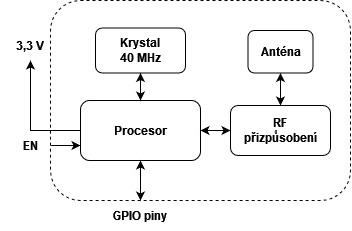
\includegraphics[scale=0.8]{obrazky/blokove_schema_MCU.jpg}
  \end{center}
  \caption[Blokové schéma mikrokontroléru ESP32-C3]{Blokové schéma mikrokontroléru ESP32-C3 \cite{ESP_C3_dtsh}.}
\end{figure}

Rozsah napájecího napětí je 3~až 3,6~V~\cite{ESP_C3_dtsh}. Jeho maximální proudový odběr je 0,5~A~\cite{ESP_C3_dtsh}. Mikrokontrolér ESP32-C3 garantuje pracovní teplotu 
od -45~°C až do 85~°C \cite{ESP_C3_dtsh}.

K~pinu 3V3, který slouží pro připojení napájecího napětí, je připojeno bateriové napětí, a také jsou k~němu připojeny kondenzátory o~hodnotě 10 $\mu$F a 100 nF dle doporučení z~dokumentace \cite{ESP_C3_dtsh}. Tyto 
kondenzátory slouží pro filtraci napájecího napětí, aby bylo vyfiltrováno případné rušení o~různých frekvencích.

Pin EN slouží pro povolení funkce mikrokontroléru. Tento pin nesmí zůstat nezapojený, tzv. floating. Jeho zapojení je převzato z~dokumentace, tj. pullup rezistor o~hodnotě 
10 k$\Omega$ a ke GND je připojen přes kondenzátor o~hodnotě 1 $\mu$F \cite{ESP_C3_dtsh}. Připojením pinu EN k~signálu GND je mikrokontrolér restartován. 

ESP32-C3 má konfigurační piny, které slouží při restartu pro určení, odkud bude načten program pro mikrokontrolér. Tyto piny musí být při restartu v~daném nastavení. 
Konfiguračními piny jsou GPIO2, GPIO8 a GPIO9. Piny GPIO8 a GPIO9 nesmí být nikdy nastaveny současně do logické nuly. 

Protože bude využito programování přes USB piny D+ a D-, tak není zapotřebí načtení z~bootloaderu a je tedy zapotřebí všechny konfigurační piny při restartu připojit do 
logické jedničky. Do logické jedničky lze připojit přes pullup rezistor. Pullup rezistory má sběrnice $I^2C$, takže na GPIO8 a GPIO9 byla připojena právě sběrnice $I^2C$.
Pin GPIO2 nebyl využit pro připojení žádného senzoru, a proto byl připojen přes pullup rezistor o~hodnotě 10 k$\Omega$ k~napájecímu napětí.

\begin{table}[!h]
  \caption[Konfigurační piny ESP32-C3]{Konfigurační piny ESP32-C3 \cite{ESP_C3_dtsh}}
  \begin{center}
  	\small
	  \begin{tabular}{|c|c|c|c|}
	    \hline
	    \textbf{Pin}	& \textbf{Výchozí}	& \textbf{Načtení programu} & \textbf{Načtení programu} \\
      \textbf{}	& \textbf{}	& \textbf{z~flash paměti} & \textbf{z~bootloaderu} \\
	    \hline
	    \textbf{GPIO2}	& Není dostupný & 1 & 1 \\ 
	    \hline
	    \textbf{GPIO8}	& Není dostupný & Nezáleží & 1 \\ 
	    \hline
	    \textbf{GPIO9} & Interní měkký pullup & 1 & 0 \\
	    \hline
	  \end{tabular}
  \end{center}
\end{table}

Na pin GPIO4 je připojeno měření napětí na baterii. Na tomto pinu je k~dispozici AD převodník se softwarově nastavitelnou hodnotou referenčního napětí \cite{ESP_C3_tech_ref}. 
Hodnota rezistorového děliče byla tedy přizpůsobena rozsahu možného měřeného napětí 0 až 700 mV. 

\begin{figure}[!h]
  \begin{center}
    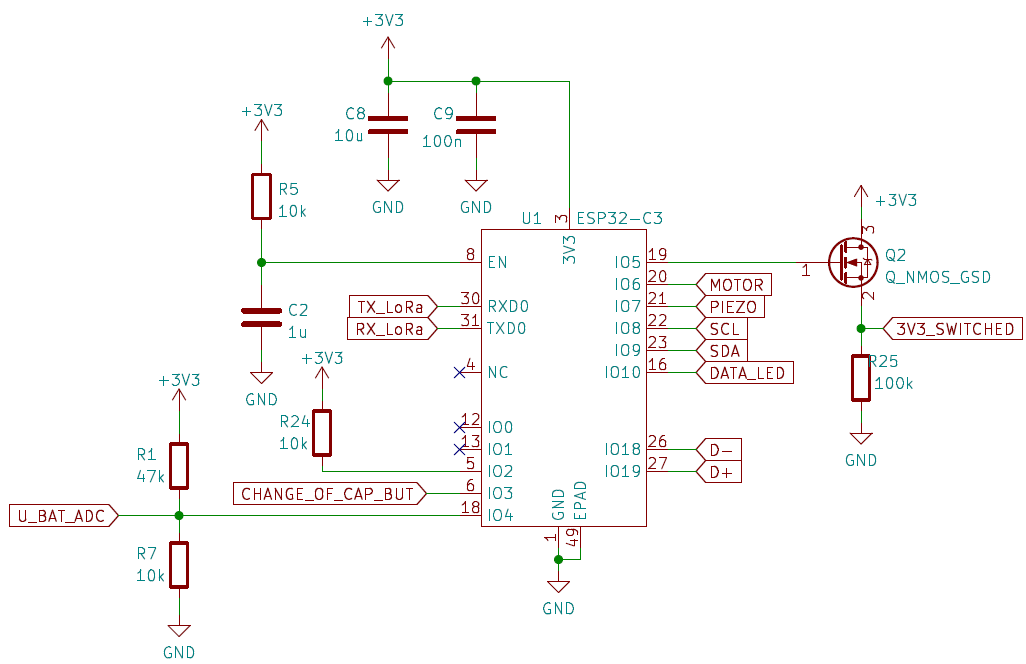
\includegraphics[scale=0.5]{obrazky/ESP32-C3.png}
  \end{center}
  \caption[Schéma zapojení mikrokontroléru ESP32-C3]{Schéma zapojení mikrokontroléru ESP32-C3.}
\end{figure}

Na piny GPIO18 a GPIO19 je možné připojení pinů D+ a D-, takže USB piny byly připojeny k~mikrokontroléru napřímo bez použití jakéhokoli převodníku \cite{ESP_C3_dtsh}. Díky 
tomu také mohou být piny sériové linky RXD0 a TXD0 využity pro připojení LoRa modulu E22-900T22D.

K~pinu GPIO5 je připojen tranzistor, který spíná napájecí napětí některým periferiím, které mají vyšší spotřebu. Napájecí napětí tak může být odpojováno například v~době,
kdy je na baterii nízké napětí. Provozní doba Univerzálního modulu se tak proudlouží a nedojde tak k~podvybití baterie a k~jejímu možnému následnému poškození. 

\section{Napájení}
Zabudování baterie přináší kompaktnost řešení a pro použití není třeba dalších komponent. Pokud je ale na táboře větší využití, tak se baterie vybije.
Na táborech většinou nebývá k~dispozici připojení k~elektrické síti, a proto je řešením powerbanka. Na Univerzálním modulu je tedy napájecí vstup USB-A pro nabíjení 
baterií přímo z~powerbanky bez nutnosti kabelu. Univerzální modul musí být koncipován tak, aby se mohla baterie nabíjet a zároveň, aby při tom mohly být Univerzální 
moduly v~provozu.

Při realizaci Univerzálního modulu byla tedy zvolena kombinace napájení pomocí baterií i~pomocí powerbanky. Článek baterie LiFePO4 byl vybrán právě kvůli již zmíněným 
vynikajícím vlastnostem. Vybraný mikrokontrolér má napájecí napětí v~rozsahu 3 až 3,6 V~\cite{ESP_C3_dtsh}. Pro funkci mikrokontroléru tedy nebude muset být použit ani 
převodník napětí. 

Napětí na baterii je měřeno pomocí děliče a připojeno na pin GPIO4, který má k~dispozici AD převodník \cite{ESP_C3_dtsh}. V~softwaru bude nastaven útlum na 0 dB, to 
odpovídá rozsahu měřeného napětí od 0 do 700 mV \cite{ESP_C3_tech_ref}.
Proto je napětí z~baterie pomocí rezistorového děliče převedeno na rozsah od 0 do 600 mV. Zde je pomocí AD převodníku napětí na baterii měřeno. Spodní rezistor děliče byl
zvolen o~hodnotě 10 k$\Omega$ a druhý byl dopočítán na hodnotu 50 k$\Omega$ podle maximálního napětí baterií LiFePO4, tj. 3,6 V. Nejbližší hodnota rezistoru je 47 k$\Omega$
\cite{rezistorova_rada}. Tomu odpovídá maximální napětí na AD převodníku 0,63 V, což je stále v~možném měřeném rozsahu. 

Při nízkém napětí baterie je díky měření možno softwarově zareagovat. Lze například odpojit napájecí napětí některým periferiím s~vyšší spotřebou, nebo signalizovat vybitou 
baterii pomocí LED blikajících červeně. 

\subsection{Nabíjecí obvod}
Nabíjecí obvody jsou závislé na konkrétním typu baterií, které budou nabíjeny. Vzhledem k~vybranému typu baterií LiFePO4 byly uvažovány pouze komerčně
dostupné integrované obvody, které jsou určeny pro nabíjení tohoto typu baterií. 

Vybraný typ baterií LiFePO4 lze nabíjet pomocí obvodu CN3058E. 

Nabíjecí obvod CN3058E je určen pro nabíjení pouze LiFePO4 baterií a lze jím nabíjet právě 1 článek tohoto typu baterie \cite{charger_dtsh}. Napájecí napětí tohoto 
nabíjecího čipu se pohybuje mezi 3,8 až 6 V~\cite{charger_dtsh}. Díky tomu lze přímo použít napětí z~USB konektoru. Když není baterie nabíjena, tak má tento nabíjecí obvod 
spotřebu 450~$\mu$A, v~nejhorším případě 600 $\mu$A \cite{charger_dtsh}. Při velikosti rezistoru, připojeného na pin ISET, 1,2~k$\Omega$ je spotřeba tohoto nabíjecího obvodu 
1 A, v~maximální hodnotě až 1,15 A~\cite{charger_dtsh}.

Když je nabíjecí obvod odpojen od napájecího napětí, tak přejde do režimu spánku \cite{charger_dtsh}. V~tomto režimu je baterie vybíjena proudem menším než 
3 $\mu$A \cite{charger_dtsh}. Tento proud je oproti klidovým proudům jiných součástek zanedbatelný, a proto nemusí být baterie od nabíjecího obvodu odpojována,
když není nabíjena. 

Nabíjecí obvod CN3058E umí také vyhodnocovat teplotu baterie a v~závislosti na tom přestávat baterii nabíjet \cite{charger_dtsh}. Tato funkce není v~zapojení
Univerzálního modulu využita, proto je pin TEMP připojen k~signálu GND \cite{charger_dtsh}.

Tento nabíjecí obvod se vyrábí ve standardizovaném pouzdře SOP8 \cite{charger_dtsh}.

\subsection{Zapojení nabíjecího obvodu}
Rezistor připojený k~pinu ISET slouží pro nastavení hodnoty nabíjecího proudu \cite{charger_dtsh}. V~tomto zapojení byl počítán pro nabíjecí proud 1 A~dle rovnice
z~dokumentace: 
\begin{equation} 
  R_{8}~=~\frac{1218}{I_{CH}}~=~\frac{1218}{1}~=~1,218~k\Omega. 
  \quad \quad \quad \quad \quad \quad \quad \quad \quad \cite{charger_dtsh}
\label{eq:I_CH}
\end{equation}

Z~výpočtu vyplývá, že rezistor by měl mít hodnotu 1,218 k$\Omega$. Nejbližší hodnota z~rezistorové řady E12 je hodnota 1,2 k$\Omega$, proto byl také zvolen rezistor 
o~této hodnotě \cite{rezistorova_rada}. Odpovídá tomu nabíjecí proud 1015 mA, který nebude mít vliv na životnost baterií. 

Vstupní a výstupní kondenzátory slouží pro filtraci zákmitů napájecího napětí a také napětí, kterým je nabíjena baterie. Hodnoty kondenzátorů byly převzaty
z~doporučení z~dokumentace, tj. 4,7 $\mu$F \cite{charger_dtsh}.

Kladný pól nabíjené baterie je připojen na pinu BAT, záporný pól je připojen k~signálu GND. Pin BAT poskytuje nabíjecí proud do baterie a zároveň poskytuje konstantní 
nabíjecí napětí. V~režimu spánku je svodový proud tohoto pinu 3 $\mu$A \cite{charger_dtsh}. 

Pin VIN slouží pro napájení vnitřního obvodu CN3058E. Je na něj přikládáno napájecí napětí z~USB, tedy 5 V. Pokud napájecí napětí klesne na napětí o~10 mV nižší, 
než je napětí na pinu BAT, tak vnitřní obvod přechází do režimu spánku \cite{charger_dtsh}. V~tomto režimu klesá proud pinu BAT na méně než 3 $\mu$A \cite{charger_dtsh}.

Tento nabíjecí obvod má možnost indikace nabíjení baterií a dokončení nabíjení. Tato indikace je realizována pomocí 2 LED připojených přes pullup rezistor. Hodnota
pullup rezistoru byla převzata z~doporučení z~dokumentace, tj. 330 $\Omega$. Červená LED indikuje nabíjení baterií a její katoda je připojena na pin /CHRG a zelená LED
indikuje dokončené nabíjení a její katoda je připojena na pin /DONE. Obě LED jsou k~napájecímu napětí připojeny anodou přes pullup rezistor R6. 

Obvod CN3058E může také měřit teplotu na nabíjené baterii. Slouží k~tomu vstupní pin TEMP. Měření probíhá pomocí odporového děliče, jehož střed je připojen na snímač 
teploty. Tento snímač je připojen na baterii. Pokud je napětí na pinu TEMP nižší než 45 \% nebo vyšší než 80 \% úrovně napájecího napětí, tak je indikována moc nízká
nebo moc vysoká teplota baterie a nabíjení je zastaveno \cite{charger_dtsh}. Jinak nabíjení pokračuje. Uzemněním pinu TEMP je funkce měření teploty deaktivována 
\cite{charger_dtsh}. V~této práci není měření teploty baterií využíváno, a proto je pin TEMP připojen ke GND. 

\begin{figure}[!h]
  \begin{center}
    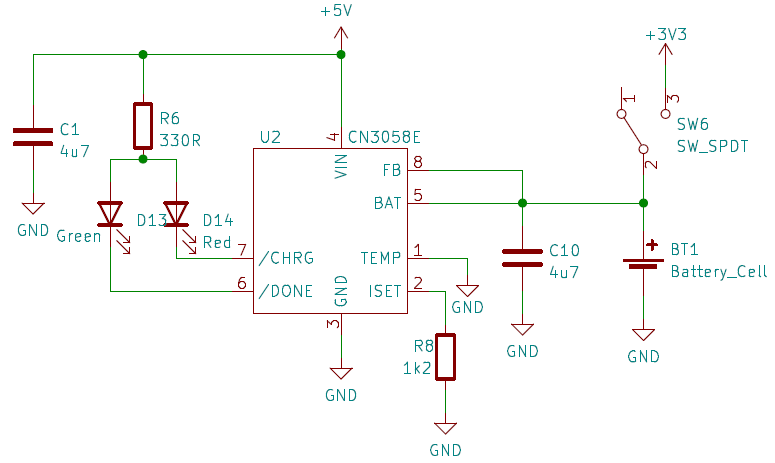
\includegraphics[scale=0.55]{obrazky/CN3058E.png}
  \end{center}
  \caption[Schéma zapojení nabíjecího obvodu CN3058E pro LiFePO4]{Schéma zapojení nabíjecího obvodu CN3058E pro LiFePO4.}
\end{figure}

\section{Senzory doteku}
V~návrhu Univerzálního modulu byla zvolena kapacitní dotyková tlačítka. Pro možnost použití uvnitř i venku jsou díky možnosti voděodolnosti 
vhodnějším řešením. Také velikost a označení tlačítka je variabilnější. Velikost může být na DPS navržena dle potřeby a potisk
v~místě tlačítka vyznačen barevně, nebo označen např. samolepkou. Odezva na dotyk bude realizována pomocí vibračního motoru.

\section{Vibrační motor}
Vibrační motory jsou založeny na principu kmitání. Motor je připevněn k~zařízení, které je kmitáním rozvibrováno. Vibrační motory jsou dnes 
nedílnou součástí mnoha elektronických zařízení včetně mobilního telefonu nebo dětských hraček. 

Schottkyho dioda D22 slouží jako ochrana proti přepětí, protože motor je indukční zátěž, takže vytváří napěťové špičky. Díky diodě je mikrokontrolér chráněn 
proti špičkovému napětí, které by se na něj mohlo dostat. Kondenzátor C25 slouží k~tomu, aby napěťové špičky eliminoval, nebo alespoň zmenšoval. 

Vibrační motor je připojen k~mikrokontroléru přes NMOS tranzistor, protože maximální výstupní proud z~pinu MCU není dostatečně velký na to, aby 
motor roztočil. Gate tranzistoru je tedy připojen k~mikrokontroléru. Tranzistor se při logické jedničce na GPIO pinu sepne a motorem protéká proud, který 
nedodává MCU, ale zdroj 3,3 V~(v~tomto případě baterie LiFePO4). Baterie tak dokáže dodat dostatek proudu, aby se motor roztočil. 

\begin{figure}[!h]
  \begin{center}
    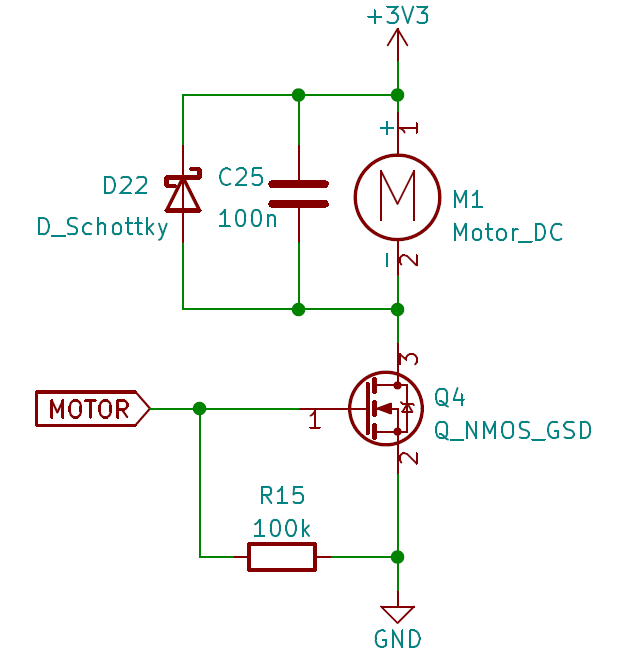
\includegraphics[scale=0.4]{obrazky/Vibracni_motor.png}
  \end{center}
  \caption[Schéma zapojení vibračního motoru]{Schéma zapojení vibračního motoru.}
\end{figure}

Pro Univerzální modul byl vybrán vibrační motor LCM1020A2945F. Tento motor má maximální požadovaný proud 120 mA \cite{vib_motor_dtsh}. Maximální 
proud, který lze odebírat z~pinu mikrokontroléru ESP32-C3, je 40 mA \cite{ESP_C3_dtsh}. Vibrační motor lze pouze spínat, nebo je možné jej připojit 
k~pinu, který dokáže generovat PWM a lze tím regulovat jeho otáčky. 

Vibrační motor slouží jako odezva na dotyk kapacitního tlačítka. 

\section{Převodník pro kapacitní tlačítka}
Mikrokontrolér ESP32-C3 nemá kapacitní vstupy, proto je zapotřebí kapacitní dotyková tlačítka připojit přes převodník. Je zapotřebí připojit 
5 tlačítek. 

Vybraný převodník AT42QT1070 dokáže pracovat ve 2 režimech. V~prvním režimu může být zapojeno maximálně 5 kapacitních tlačítek, která jsou připojena
k~pinům KEY0 až KEY4. Jako výstup se používají piny OUT0 až OUT4. Každé tlačítko má tedy svůj výstup, který může být připojen k~GPIO pinům mikrokontroléru
nebo k~nim mohou být připojeny např. LED \cite{conv_cap_but_AT42QT1070_dtsh}. 

Druhý režim je využitelný pouze v~případě, je-li převodník připojen k~MCU. V~tomto případě může být k~převodníku připojeno až 7 kapacitních tlačítek, 
která jsou připojena na pinech KEY0 až KEY6. Převodník poté komunikuje s~MCU pomocí komunikační sběrnice $I^2C$ \cite{conv_cap_but_AT42QT1070_dtsh}. 
Z~registru převodníku lze poté vyčíst stavy daných kapacitních dotykových tlačítek. 

Jelikož je v~tomto návrhu Univerzálního modulu využit mikrokontrolér, který podporuje komunikaci po sběrnici $I^2C$, tak bylo využito zapojení právě s~tímto typem 
komunikace. Díky tomu budou využity pouze 2 GPIO piny mikrokontroléru ESP32-C3 a ne 5 GPIO pinů, které by byly zapotřebí při zapojení bez komunikace pro
sběrnici $I^2C$. Komunikační sběrnice $I^2C$ vyžaduje pullup rezistory, proto byly mezi napájecí napětí a piny SDA a SCL převodníku AT42QT1070 
přidány rezistory R17 a R18 o~hodnotě 10 k$\Omega$. To znamená, že komunikační sběrnice $I^2C$ je aktivní v~logické nule. 

Kapacitní tlačítka jsou připojena přes rezistory R19 až R23 k~převodníku AT42QT1070. Tyto rezistory jsou připojeny sériově a slouží ke snížení šumu, 
omezení elektrostatických výbojů a potlačení radiofrekvenčního rušení \cite{conv_cap_but_AT42QT1070_dtsh}. Doporučená hodnota rezistorů je mezi 
4,7k$\Omega$ a 20 k$\Omega$ \cite{conv_cap_but_AT42QT1070_dtsh}. Byla zvolena střední hodnota z~doporučeného rozsahu, tj 10 k$\Omega$.

\begin{figure}[!h]
  \begin{center}
    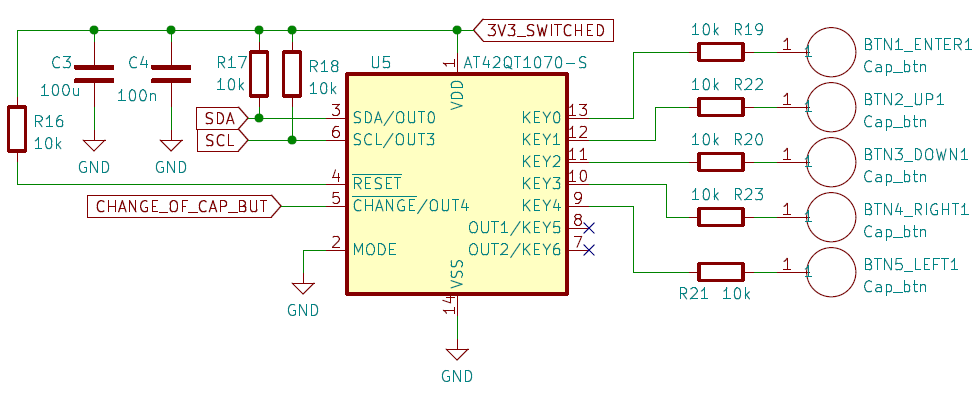
\includegraphics[scale=0.55]{obrazky/AT42QT1070.png}
  \end{center}
  \caption[Zapojení převodníku AT42QT1070 pro kapacitní tlačítka]{Zapojení převodníku AT42QT1070 pro kapacitní tlačítka.}
\end{figure}

Převodník má kondenzátory C3 a C4 připojeny na napájecím pinu vůči GND, aby nebyly případné proudové špičky přivedeny na napájení převodníku. Rezistory
R17 a R18 slouží jako pullup rezistory při komunikaci pomocí sběrnice $I^2C$ s~mikrokontrolérem EP32-C3. Na piny KEY0 až KEY4 jsou připojena kapacitní 
dotyková tlačítka. 

Pin MODE je připojen k~signálu GND, protože převodník je provozován v~režimu komunikujícím přes $I^2C$ sběrnici \cite{conv_cap_but_AT42QT1070_dtsh}.

Pin /CHANGE je připojen k~GPIO pinu mikrokontroléru. Slouží pro indikaci změny stavu některého z~připojených tlačítek \cite{conv_cap_but_AT42QT1070_dtsh}. 
Signál z~tohoto pinu lze tedy využít jako indikátor vyvolání přerušení pro obsluhu tlačítek. 

Pin KEY0 může být také využit pro tzv. ochrannou zónu \cite{conv_cap_but_AT42QT1070_dtsh}. Tento kanál slouží pro zabránění falešným 
detekcím \cite{conv_cap_but_AT42QT1070_dtsh}. Tento pin je citlivější než ostatní \cite{conv_cap_but_AT42QT1070_dtsh}. Ochranná zóna by měla být také větší 
než použitá tlačítka. Této funkce nebylo do prototypu DPS využito. 

\section{Světelná signalizace}
Pro realizaci signalizace přítomnosti napájecího napětí byly vybrány neprogramovatelné LED. Zelené LED byly vybrány dvě, jedna pro 
indikaci přítomnosti napětí 5~V~a druhá pro indikaci přítomnosti napětí 3,3 V~z~baterií. Tyto LED budou použity pouze na prototypu 
pro ulehčení oživování. 

Pro realizaci světelné signalizace pro hry byly vybrány inteligentní programovatelné LED typu WS2812C. Bylo jich použito 12, protože 
z~dvanácti LED lze jednoduše zhotovit ciferník pro odpočítávání času a také je lze rozdělit na segmenty na poloviny, třetiny nebo čtvrtiny. 

\begin{figure}[!h]
  \begin{center}
    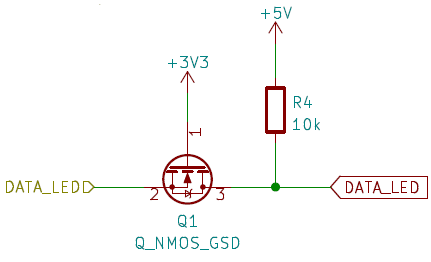
\includegraphics[scale=0.6]{obrazky/prevodnik_urovni_pro_WS2812C.png}
  \end{center}
  \caption[Zapojení převodníku úrovní pro WS2812C]{Zapojení převodníku úrovní pro WS2812C.}
\end{figure} 

Komunikační napěťová úroveň logické jedničky těchto LED by měla být alespoň na úrovni 70 \% napájecího napětí \cite{WS2812C_dtsh}. 
Protože použitý mikrokontrolér ESP32-C3 má komunikační napěťovou úroveň logické jedničky jeho napájecího napětí, což je 3 až 3,6 V, 
tak je zapotřebí využít převodník napěťové úrovně \cite{ESP_C3_dtsh}. Komunikace je v~tomto případě pouze jednosměrná, 
to znamená, že mikrokontrolér posílá data do LED, ale LED neposílají žádná data do mikrokontroléru. Převodník je realizován unipolárním 
NMOS tranzistorem 
a~jedním pullup rezistorem. Rezistor je připojen k~napájecímu napětí inteligentních LED WS2812C. 
Tranzistor Q1 má gate připojený k~napájecímu napětí MCU. Pokud bude mikrokontrolér do LED posílat logickou jedničku, tak bude rozdíl
mezi gate a~source 0 V. Tím pádem bude tranzistor uzavřený a tím se přes rezistor R4 připojí k~LED jejich napájecí napětí. Toto napětí 
je pro inteligentní LED logickou jedničkou. Pokud bude MCU posílat logickou nulu, tedy 0 V, tak je rozdíl napětí mezi gate a~source 
napájecí napětí mikrokontroléru. Tranzistor je tedy otevřený, a tím se napětí 0 V~dostane k~inteligentním LED a na rezistoru R4 se objeví
úbytek napětí o~velikosti napájecího napětí inteligentních LED. Napětí 0 V~je logickou nulou i pro inteligentní LED. Tento převodník
je určen pouze pro komunikaci jedním směrem. 

\begin{figure}[!h]
  \begin{center}
    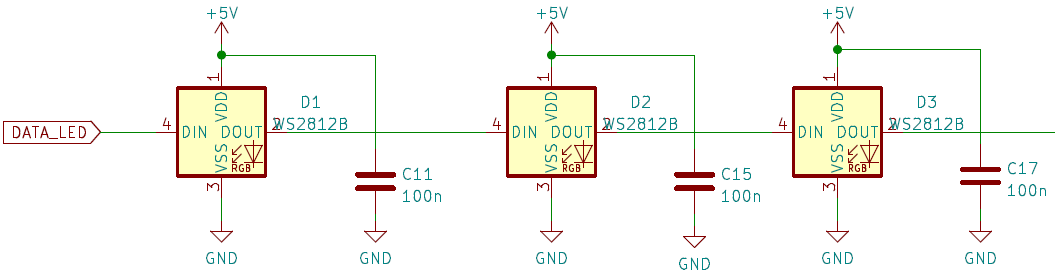
\includegraphics[scale=0.5]{obrazky/WS2812C.png}
  \end{center}
  \caption[Zapojení inteligentních LED WS2812C]{Zapojení inteligentních LED WS2812C.}
\end{figure}

Kondenzátor u~každé LED slouží pro filtraci napájecího napětí. 

Tyto programovatelné LED mají maximální spotřebu 5 mA na jeden kanál. Při zapnutí všech kanálů (svícení bílou) je maximální
spotřeba jedné LED 15 mA \cite{WS2812C_dtsh}. Pokud LED nesvítí, tak je její maximální klidový proud 0,3 mA \cite{WS2812C_dtsh}.
Při použití 12 LED je tedy maximální odběr všech LED 180 mA.

Pro napájení těchto inteligentních LED je zapotřebí napětí v~rozsahu 4,5 až 5,5~V~\cite{WS2812C_dtsh}. 
Použité baterie LiFePO4 mají napětí pouze 3,2 V, proto je zapotřebí použít zvyšovač napětí na 5 V. 

\subsection{Zvyšovač napětí pro programovatelné LED}
Z~komerčně dostupných integrovaných obvodů byl hledán zvyšovač napětí, který vytváří z~napětí 3,3 V~napětí 5 V~a může přitom dodávat do výstupu proud alespoň 200 mA. 
Maximální odběr všech dvanácti potřebných inteligentní LED má maximální odběr 180 mA. S~rezervou je tedy zapotřebí proud alespoň 200 mA. Nalezené obvody, které vyhovují 
těmto parametrům jsou LT1930 a MCP1640. 

Obvod LT1930 v~doporučeném zapojení při vstupním napětí 3,3V vytváří výstupní napětí o~hodnotě 5 V~s~maximálním odběrem proudu 480 mA \cite{LT1930_dtsh}. Napájecí napětí 
tohoto obvodu je v~rozsahu 2,45 V~až 16 V, což vyhovuje napájecímu napětí z~baterií LiFePO4 \cite{LT1930_dtsh}.

Obvod MCP1640 v~doporučeném zapojení s~rozsahem vstupního napětí 3 až 4,2~V~vytváří výstupní napětí o~hodnotě 5 V~s~maximálním odběrem proudu 300~mA \cite{MCP1640_dtsh}.

Byl vybrán zvyšovač napětí LT1930, díky své lepší dostupnosti v~této době nedostatku čipů, a také dokáže do výstupu dodat vyšší proud. Zapojení obou čipů je téměř totožné. 

Pin /SHDN slouží k~zapínání a vypínání obvodu. Pomocí přiloženého napětí 2,4 V~a více na tento pin je obvod zapnut \cite{LT1930_dtsh}. Pin SW slouží pro  připojení cívky, 
případně diody, aby se snížilo elektromagnetické rušení \cite{LT1930_dtsh}. 

\begin{figure}[!h]
  \begin{center}
    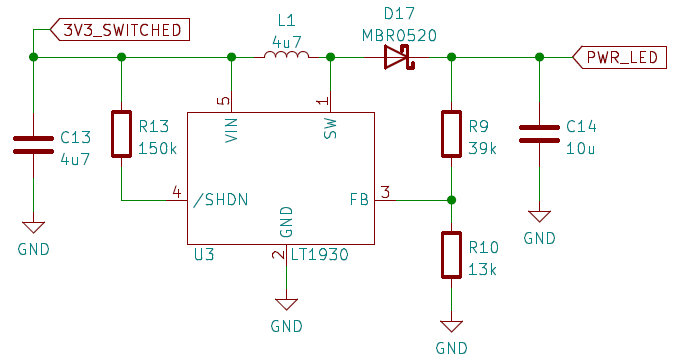
\includegraphics[scale=0.6]{obrazky/LT1930.png}
  \end{center}
  \caption[Zapojení zvyšovače napětí LT1930]{Zapojení zvyšovače napětí LT1930.}
\end{figure}

Shottkyho dioda byla vybrána dle doporučení z~dokumentace. Byla vybrána dioda typu MBR0520, protože maximální napětí na diodě nepřekročí 20 V~a protékající proud nepřesáhne 
0,5 A~\cite{LT1930_dtsh}.

Byla vybrána cívka, která odpovídá doporučení z~dokumentace. Přesný typ, který byl v~dokumentaci zmíněn, nebyl k~dispozici, a proto byl vybrán typ velmi podobný a vlastnostmi 
srovnatelný. Cívka CDRH3D18NP-4R7NC má feritové jádro, které je pro funkci požadováno \cite{LT1930_dtsh}, \cite{civka_dtsh}. Pro zvyšovač napětí LT1930 by měl být proud, který cívkou může protékat, 
alespoň 1A a její indukčnost by měla být 4,7 $\mu$H nebo 10 $\mu$H \cite{LT1930_dtsh}. Vybraná cívka má indukčnost 4,7 $\mu$H \cite{civka_dtsh}. Proud, který jí může protékat, je 1,35 A~a její rozměry 
jsou 3,8 $\times$ 3,8 $\times$ 2 mm \cite{civka_dtsh}.

Pin FB slouží  pro zapojení zpětné vazby napětí na baterii. Jeho referenční napětí musí být nastaveno v~rozmezí 1,240~V~až 1,270 V, typická hodnota je však 1,255~V~\cite{LT1930_dtsh}. 
Pro výstupní napětí 5 V~byl zvolen spodní rezistor R10 o~hodnotě 13 k$\Omega$ z~rezistorové řady E24 \cite{rezistorova_rada}. Řada E24 byla zvolena kvůli požadované přesnosti
napětí na pinu FB obvodu LT1930. Napětí na rezistoru R10 musí být tedy 1.255 V. Na horním rezistoru R9 je tedy úbytek napětí 3,745 V. Pomocí trojčlenky byla dopočítána hodnota 
rezistoru R9 dle rovnice:
\begin{equation} 
  R_{9}~=~\frac{R_{10}~\cdot~U_{R9}}{U_{R10}}~=~\frac{13~\cdot~3,745}{1,255}~=~38,79~\:k\Omega. 
  \quad
\label{eq:R9}
\end{equation}

Nejbližší hodnota rezistoru z~rezistorové řady E24 je 39 k$\Omega$ \cite{rezistorova_rada}. Reálná hodnota napětí na rezistoru R10, tj. napětí na pinu FB byla dopočítána
dle rovnice:
\begin{equation} 
  U_{R10}~=~\frac{U_{OUT}}{R_{9}~+~R_{10}}~\cdot~R_{10}~=~\frac{5}{39~+~13}~\cdot~13~=~1,25~V. 
  \quad
\label{eq:UR10}
\end{equation}

Napětí 1,25 V~je v~povoleném rozmezí napětí na pinu FB. 

Přesné výstupní napětí se spočítá podle vzorce:
\begin{equation} 
  U_{OUT}~=~U_{FB}~\cdot~(1~+~\frac{R_{9}}{R_{10}})~=~1,25~\cdot~(1~+~\frac{39}{13})~=~5~V. 
  \quad \quad \quad \quad \cite{LT1930_dtsh}
\label{eq:VOUT_LT1930}
\end{equation}

\section{Zvuková signalizace}
Zvuková signalizace může sloužit například pro potvrzení správnosti hesla, možnosti odejít na další stanoviště, vypršení času pro daný úkol a mnoho dalších. 

Jako zvuková signalizace bylo vybráno piezo s~vlastním oscilátorem typu \\BMT1205XH7.5 \cite{piezo_dtsh}. Maximální odebíraný proud vybraného pieza je 30 mA a rezonanční frekvence 
je 2,3 kHz \cite{piezo_dtsh}. Intenzita zvuku pieza je ve vzdálenosti 10 cm od něj minimálně 83 dB \cite{piezo_dtsh}.

\begin{figure}[!h]
  \begin{center}
    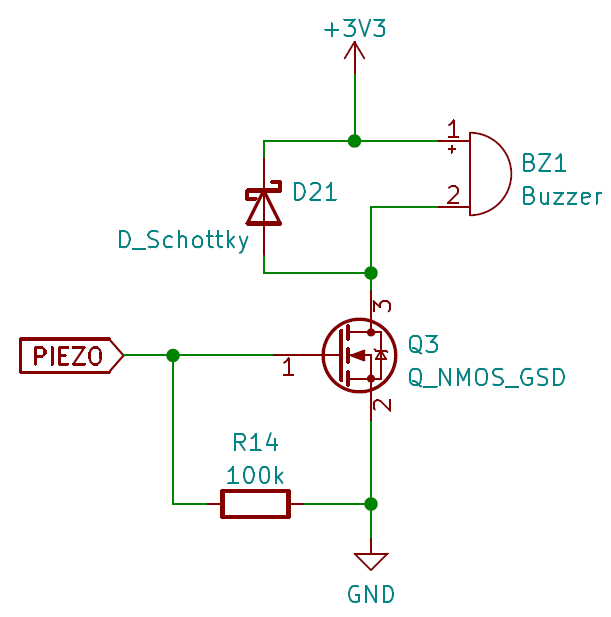
\includegraphics[scale=0.45]{obrazky/piezo.png}
  \end{center}
  \caption[Schéma zapojení pieza]{Schéma zapojení pieza.}
\end{figure}

\section{Konektor}
Jako programovací a zároveň nabíjecí konektor byl zvolen konektor USB-C. Tento konektor je v~dnešní době velmi rozšířený a jeho použití se v~následující době stále rozšiřuje. 

Konektoru USB-C je využíván pouze jako standardní a dostupný konektor, který je mezi běžnou
populací rozšířený a v~následujících letech se bude rozšiřovat stále více. Je využito standardního jmenovitého napětí 5 V~pro nabíjení baterií a nadále jsou také využity 
piny D+ a D-, které jsou využity pro komunikaci při programování. 

Konektor USB-C je robustní a oboustranný, díky čemuž nebude docházet k~tak častému poškození, jak by mohlo být např. u~konektoru Micro USB. Při používání běžnou veřejností
se jedná o~vítaný bonus. 

Vybraný mikrokontrolér ESP32-C3 umožňuje komunikaci přímo po USB protokolu a není díky tomu zapotřebí žádného převodníku pro komunikaci \cite{ESP_C3_dtsh}.

\begin{figure}[!h]
  \begin{center}
    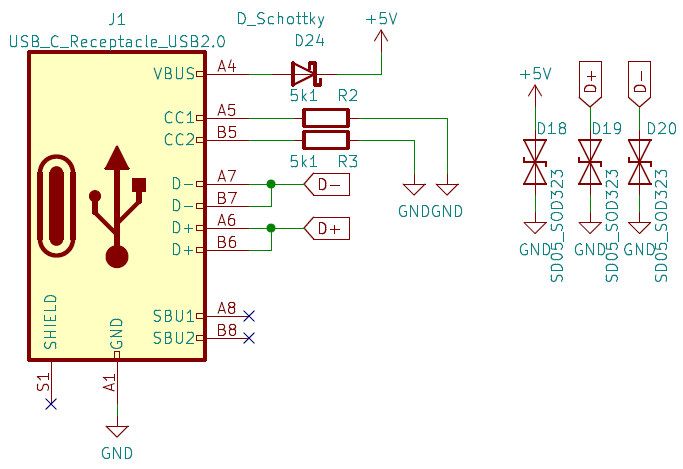
\includegraphics[scale=0.5]{obrazky/USB_C.png}
  \end{center}
  \caption[Zapojení konektoru USB-C]{Zapojení konektoru USB-C.}
\end{figure}

Připojené Shottkyho diody k~napájecímu napětí slouží pro zadržení případného zpětného proudu. Shottkyho diody jsou dimenzovány na proud, který odebírá celé zařízení. Vybrané 
Shottkyho diody  B5819W mají maximální napětí 20 V, jmenovitý proud 1 A~a maximální špičkový proud 9 A~\cite{shotky_dtsh}.

Transily připojené k~napájecímu pinu a ke komunikačním pinům D+ a D- slouží k~ochraně proti přepětí a elektrostatickým výbojům o~velikosti až 30 kV. 

Rezistory o~hodnotě 5,1 k$\Omega$ na pinech CC1 a CC2 slouží pro signalizaci, že je k~USB-C připojeno zařízení. Dle standardu USB-C totiž nabíječka bez 
připojení těchto rezistorů nesmí připojit napájecí napětí 5 V~na pin VBUS \cite{USB-C}. 

Pro napájení pomocí powerbanky bez potřeby kabelu slouží konektor USB-A. 

\begin{figure}[!h]
  \begin{center}
    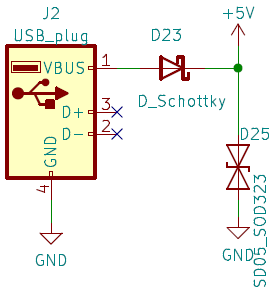
\includegraphics[scale=0.6]{obrazky/USB_A.png}
  \end{center}
  \caption[Zapojení konektoru USB-A]{Zapojení konektoru USB-A.}
\end{figure}

\section{Výsledné zapojení}
Pro realizaci Univerzálního modulu byly vybrány následující komponenty: mikrokontrolér ESP32-C3, baterie LiFePO4, nabíjecí obvod CN3056E, konektory USB-C a USB-A,
kapacitní tlačítka s~převodníkem AT42QT1070, inteligentní LED WS2812C s~převodníkem napětí LT1930, piezo BMT1205XH7.5, vibrační motor LCM1020A2945F a~LoRa modul 
E22-900T22D. LoRa modul komunikuje 
s~mikrokontrolérem pomocí sběrnice UART, převodník pro kapacitní tlačítka pomocí sběrnice $I^2C$ a programování bude probíhat pomocí USB pinů D+ a D-. Vše je 
zapojeno dle následujícího blokového schématu. 

\begin{figure}[!h]
  \begin{center}
    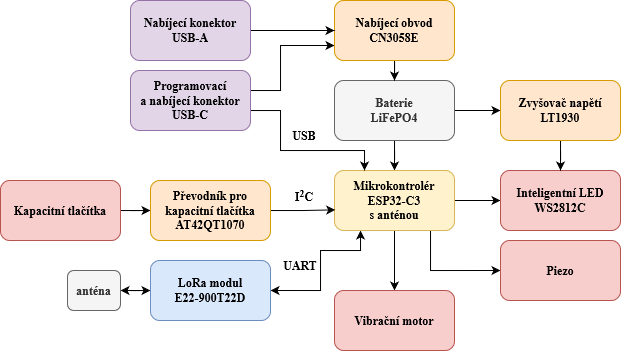
\includegraphics[scale=0.65]{obrazky/vysledne_blokove_schema.png}
  \end{center}
  \caption[Blokové schéma Univerzálního modulu]{Blokové schéma Univerzálního modulu.}
\end{figure}


\chapter{Návrh DPS}
Byl zvolen kruhový tvar desky s~průměrem téměř 15 cm a s~výběžkem USB-A pro připojení powerbanky. Deska plošného spoje byla navržena v~programu KiCad 6.0 a~má 2 vrstvy mědi. 
Některé součástky jsou natočeny tak, aby byly co nejvíce na kraji kulaté DPS.

Komunikační dráhy jsou vedeny o~tloušťce 0,150 mm a napájecí dráhy jsou vedeny o~tloušťce 0,5 mm. Celý návrh byl přizpůsoben výrobním možnostem firmy JLCPCB, kde byla DPS vyrobena.

Při návrhu DPS byla dodržována pravidla a konvence dobrého návrhu DPS.

V~oblasti antény od ESP32-C3 mikrokontroléru nejsou taženy žádné dráhy, ani pod ní není rozlitá žádná měď. Je to z~důvodu zaručení většího dosahu signálu a pro snížení rušení. 

Filtrační kondenzátory jsou vždy umístěny co nejblíže pouzdrům daných čipů. Shottkyho diody a transily jsou umístěny v~blízkosti USB konektorů. Rozmístění součástek kolem zvyšovače napětí 
je provedeno dle doporučení z~dokumentace. 

Komunikační piny D+ a D- pro programování jsou taženy jako diferenciální pár.

\section{Kapacitní tlačítka} 
Byl požadavek na 5 tlačítek. Jedno tlačítko je uprostřed a slouží jako hlavní tlačítko. U~her bude používáno např. jako registrace průchodu místem apod. Bude tedy nejčastěji
používáno a zároveň může být stisknuto, když hráč běží, takže by mělo být co nejjednodušeji stisknutelné. Proto bylo navrženo větší než zbylá tlačítka. Konkrétně má 
čtvercový tvar se zaoblenými rohy s~rozměry 5~$\times$~5~cm. Ostatní tlačítka slouží například jako směrovky, nebo pro vyklikávání nějakého kódu, aby získali nějakou informaci. 
Slouží tedy primárně, když hráč u~Univerzálního modulu stojí, nebo sedí, a vyklikává. Díky tomu mohou být tlačítka menší než hlavní tlačítko, konkrétně mají 2~$\times$~2~cm 
a jsou taktéž čtvercová se zaoblenými rohy. Tato tlačítka jsou proto umístěna po stranách hlavního tlačítka.

V~oblastech kapacitních tlačítek nejsou umístěny žádné další součástky a v~jejich okolí je rozmístěna země kvůli odstínění. 

Pod spodním tlačítkem je ze spodní strany umístěno pouzdro na baterii. Kdyby bylo pouzdro až pod tlačítkem, musel by se ještě hodně zvětšit průměr DPS. Pokud by se při testování 
prototypu ukázalo, že kvůli umístění pouzdra baterie dochází k~rušení tlačítka, tak dojde při výsledné verzi DPS k~posunutí pouzdra baterie. 

\section{LED}
Po obvodu DPS je poté rovnoměrně rozmístěno do kruhu všech 12 programovatelných LED. Takto rozmístěné LED mohou zobrazovat např. podíl uběhnutého času. Dvanáct LED bylo zvoleno 
z~důvodu možnosti rozdělení na 2, 3 nebo i 4 segmenty. Na dvanácti LED v~kruhu lze také zobrazovat čas.

\section{Ostatní součáskty}
Ze zadní strany DPS je umístěna veškerá řídicí elektronika. Ve spodní straně je umístěno pouzdro s~baterií LiFePO4 a v~jeho blízkosti je umístěn nabíjecí obvod. V~levém 
spodním rohu je poté umístěn konektor USB-C, který slouží pro nabíjení baterie a zároveň pro programování. Nad pouzdrem pro baterii je umístěn zvyšovač napětí pro programovatelné 
LED a nedaleko jsou LED diody indikující přítomnost napájecího napětí 3,3 V~a 5 V. Ze zadní strany je v~levé horní části umístěn mikrokontrolér ESP32-C3 a v~pravé horní části 
LoRa modul. Nad tlačítky je umístěn převodník pro kapacitní tlačítka AT42QT1070-S.

Otvory pro připojení vypínače jsou umístěny u~konektoru USB-C a otvory pro připojení vibračního motoru jsou umístěny mezi LoRa modulem a vrchním tlačítkem. 

Z~přední strany DPS je také umístěn bzučák. 

\chapter{Osazení, oživení a testování DPS}
Výrobní podklady byly vygenerovány pomocí programu Kikit. Deska byla vyrobena u~firmy JLCPCB, protože je bezkonkurenčně nejlevnější a její dodání je rychlé a~bezproblémové. 
Jejich výrobky také dosahují vysoké kvality. 

\begin{figure}[!h]
  \begin{center}
    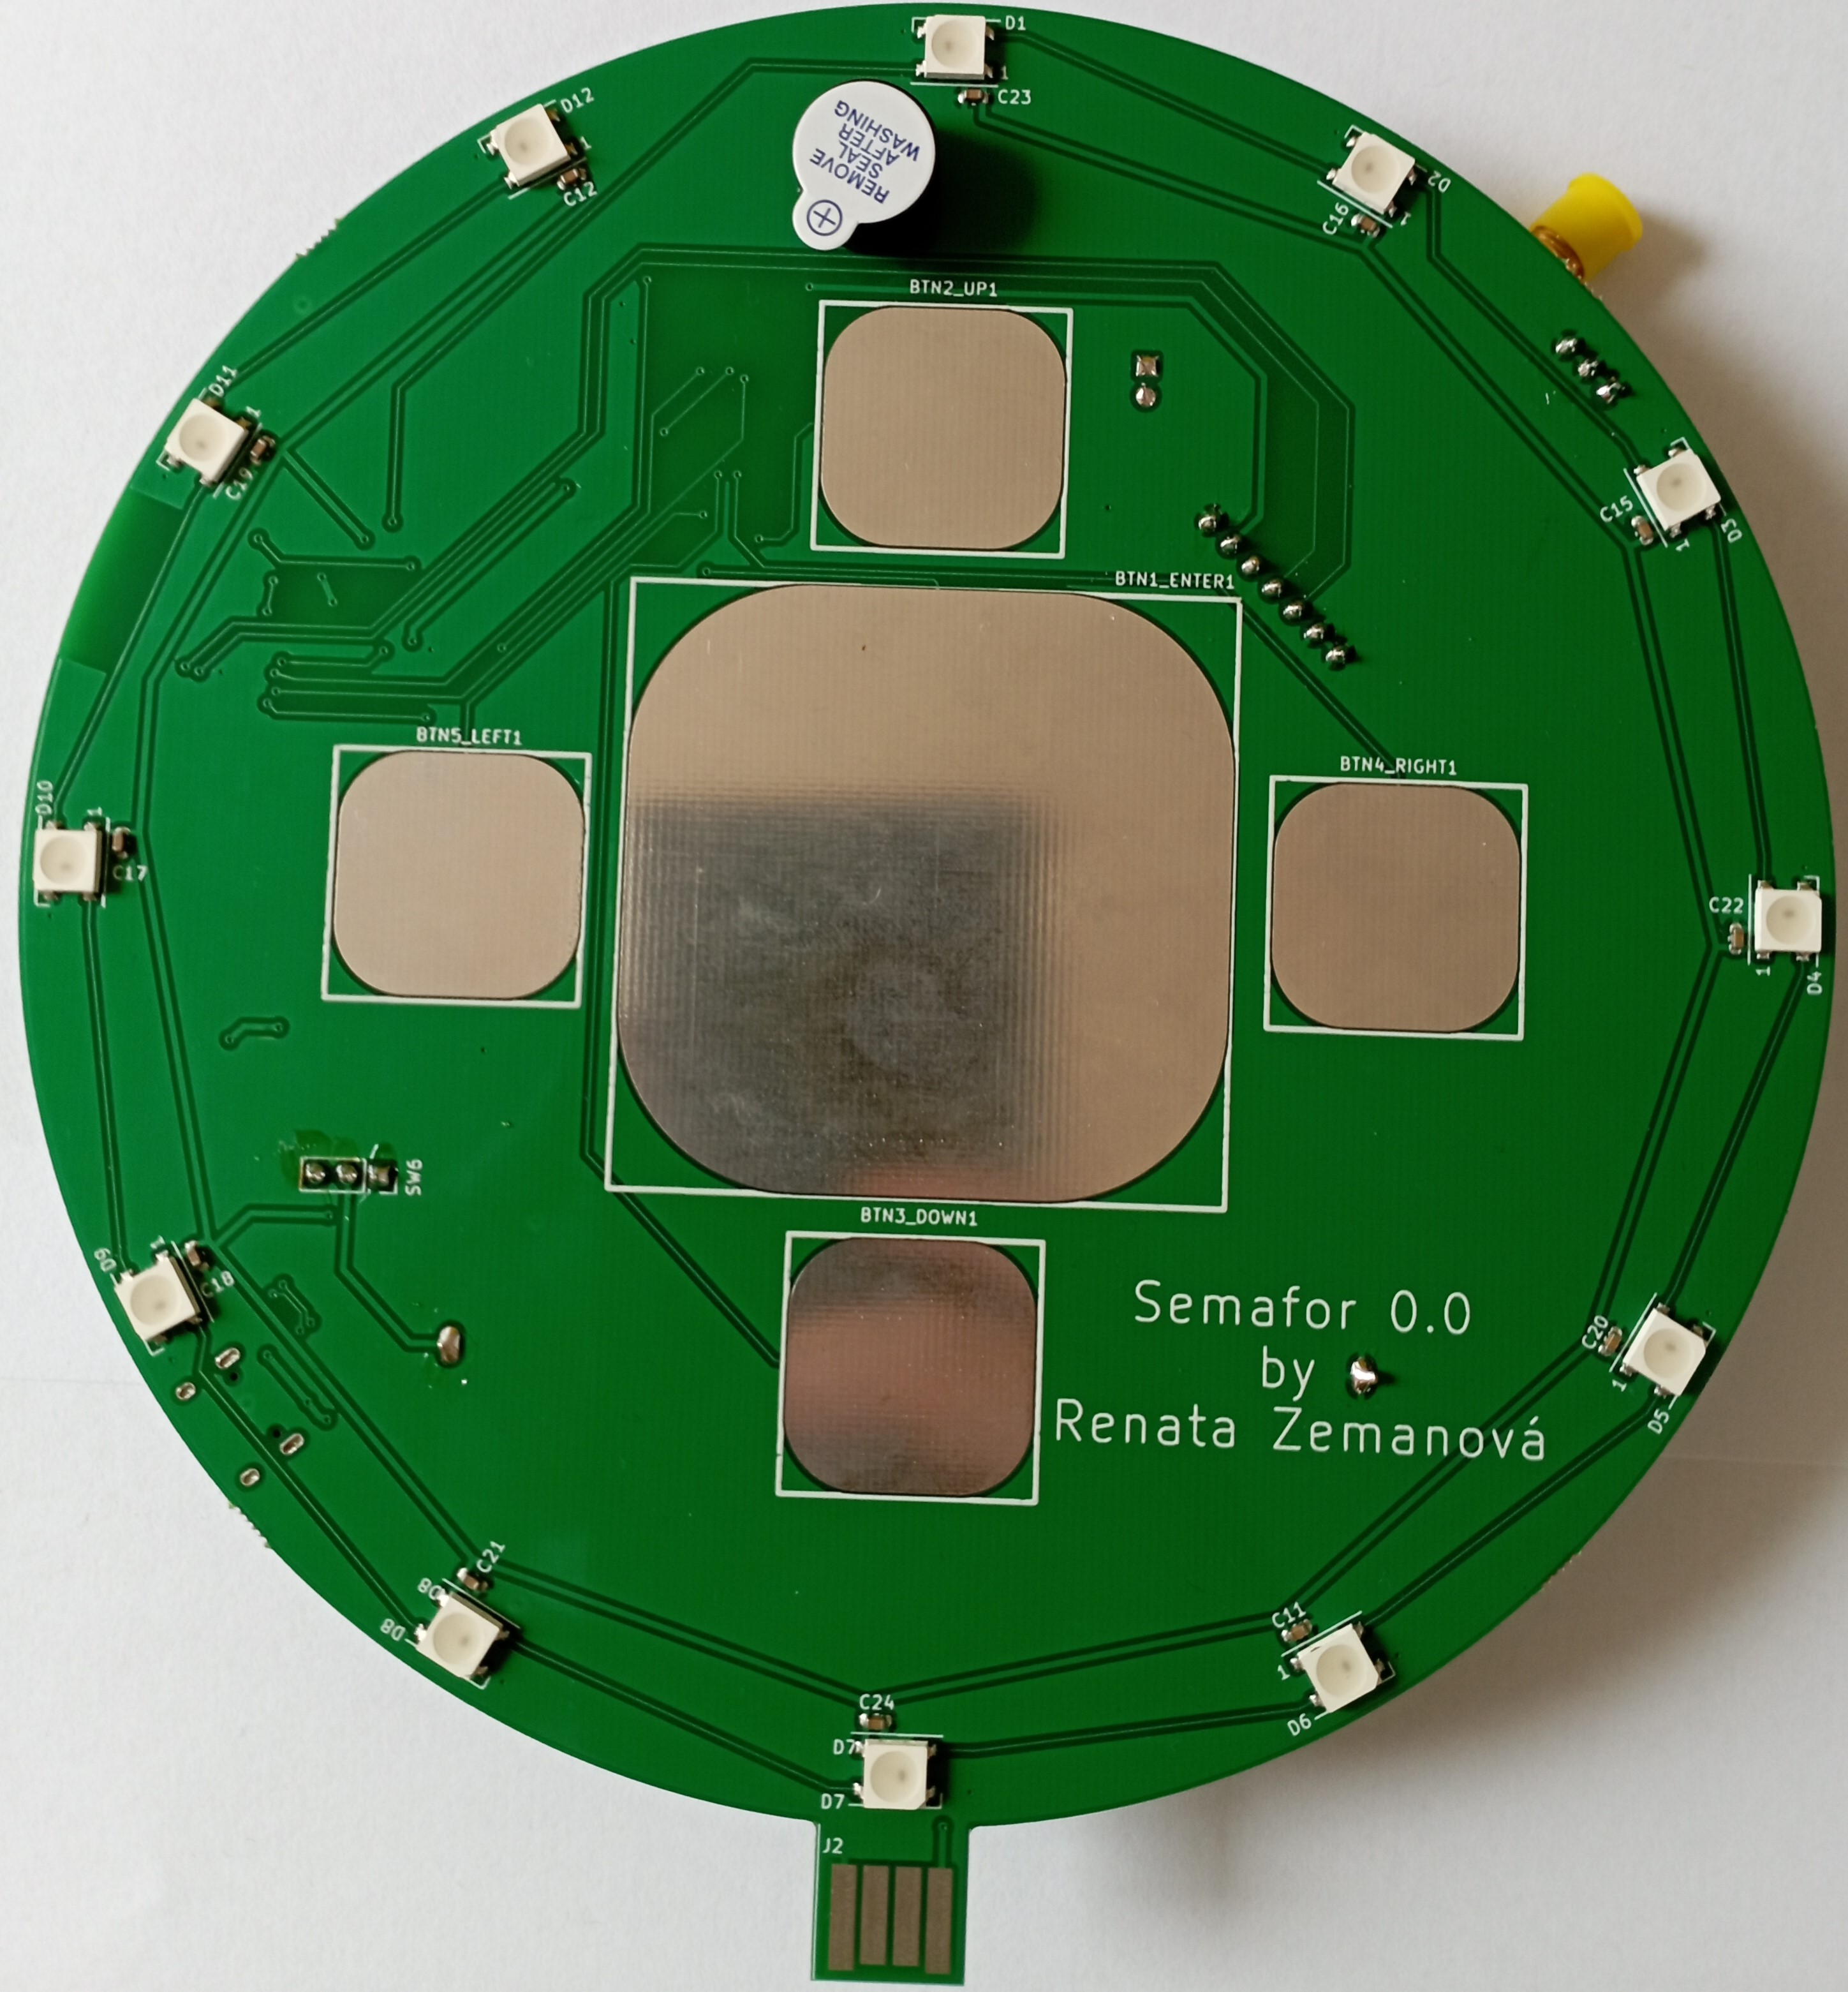
\includegraphics[scale=0.15]{obrazky/DPS_prototyp_top.jpg}
  \end{center}
  \caption[Výsledná DPS prototypu - přední strana]{Výsledná DPS prototypu - přední strana.}
\end{figure}

DPS byla taktéž strojově osazena u~firmy JLCPCB. Z~důvodu nedostupnosti některých součástek byly některé komponenty zakoupeny v~jiných obchodních řetězcích a doosazeny ručně. 
Jednalo se o~držák na baterie, piezo, kondenzátor C3 v~pouzdře 0805 o~hodnotě 100 $\mu$F, čip pro kapacitní tlačítka AT42QT1070, vypínač a LoRa modul. 

Nebyl sehnán přesný typ držáku, pro který byl Univerzální modul navržen. Proto byly nožičky držáku roztaženy, aby byla jejich rozteč zvětšena a mohlo dojít k~zapájení. Do finální 
verze byla rozteč zmenšena, aby došlo k~zapájení bez větších problémů. U~pieza také chybělo 
označení polarity. Do finální verze bylo tedy přidáno do popisové vrstvy plus u~správného vývodu. Vypínač byl kvůli testovacím účelům realizován pinheady a na ně byla nasazena 
propojka. Na místo LoRa modulu byly připájeny dutinky a LoRa modul byl pouze zasunut do dutinek. Hlavním důvodem byla cena tohoto modulu. LoRa modul bude z~prototypu přesunut 
na finální výrobek a nedojde tak k~plýtvání součástek ani peněz.

\begin{figure}[!h]
  \begin{center}
    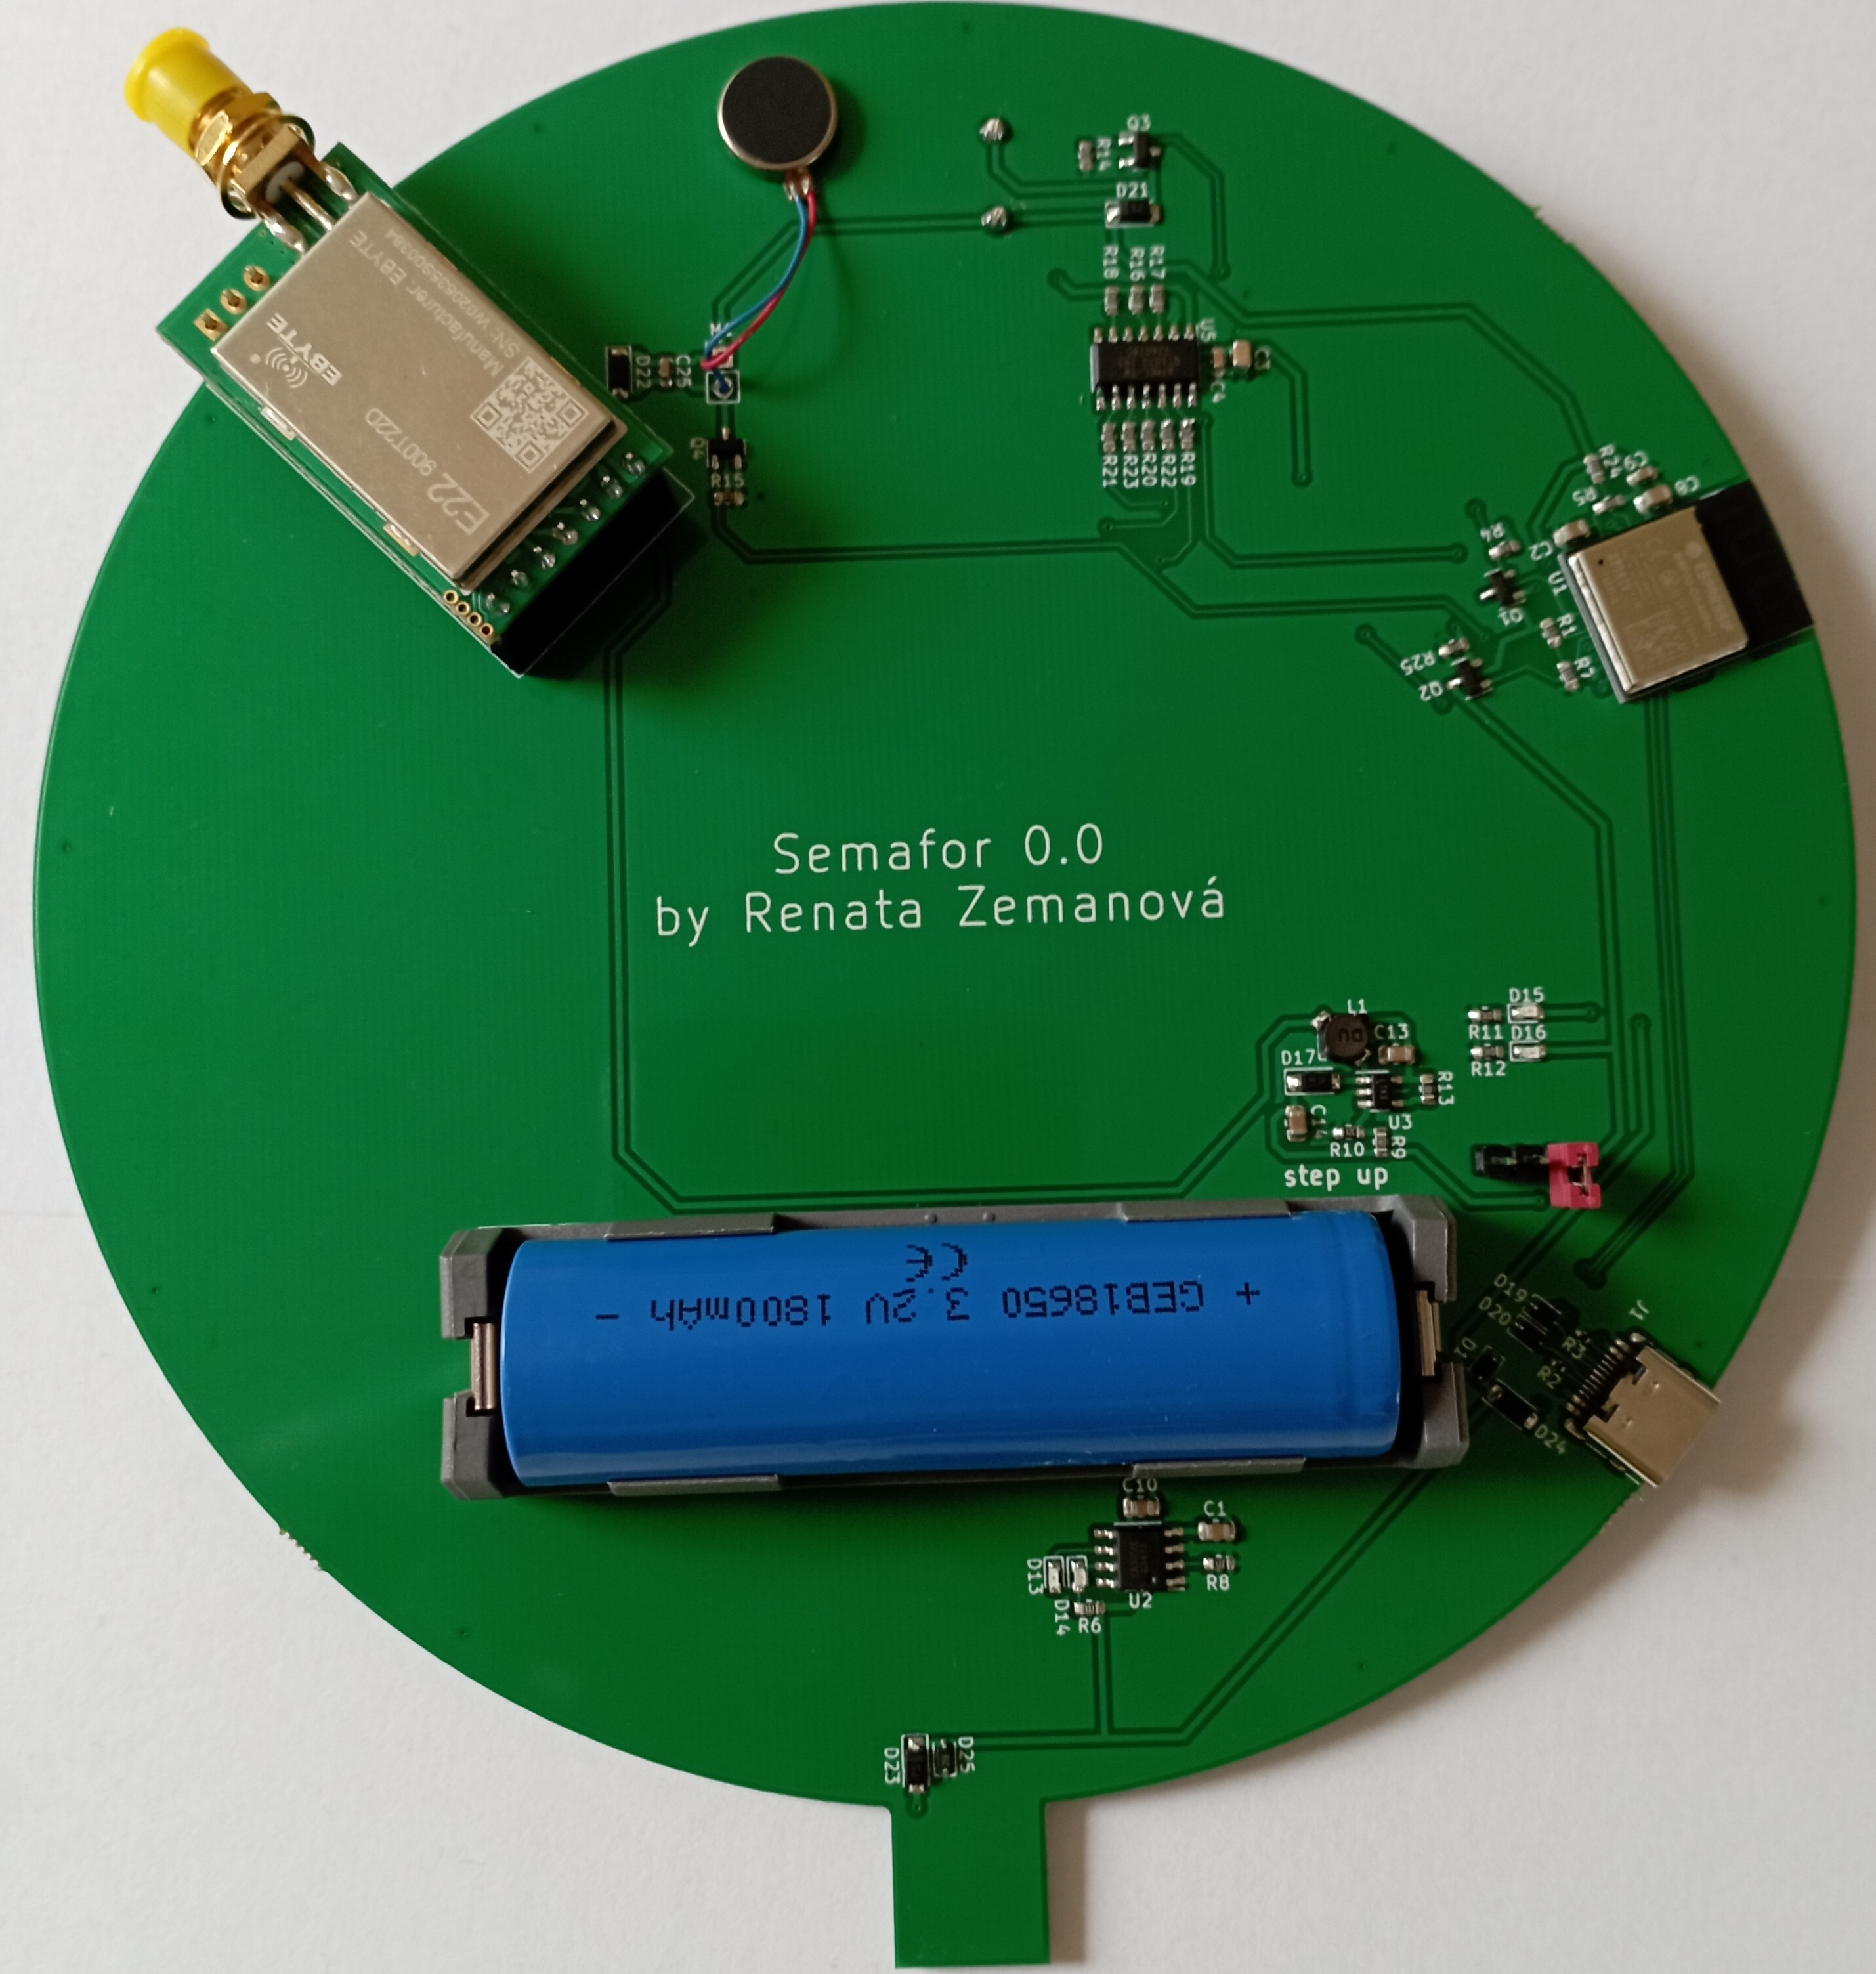
\includegraphics[scale=0.15]{obrazky/DPS_prototyp_bottom.jpg}
  \end{center}
  \caption[Výsledná DPS prototypu - zadní strana]{Výsledná DPS prototypu - zadní strana.}
\end{figure}

\section{Oživení}
Po připájení všech součástek byla do pouzdra vložena baterie LiFePO4 a DPS byla pomocí propojky zapnuta. Po zapnutí DPS se rozsvítila LED indikující přítomnost bateriového napětí 3,3 V. 
Po připojení konektoru USB-C k~napájecímu napětí se rozsvítila i LED indikující napětí 5 V. Také se rozsvítila červená LED indikující nabíjení baterie. Baterie byla pod dohledem 
nabíjena v~DPS. Nedošlo k~zahřátí DPS ani baterie a po čase se u~nabíjecího obvodu rozsvítila místo červené LED zelená LED. Tato LED indikuje plně nabitou baterii. Na plně nabité 
baterii bylo multimetrem naměřeno napětí 3,4 V. Nabíjecí obvod byl tedy otestován a bylo zjištěno, že funguje správně. 

Při měření napětí bylo zjištěno, že napájecí napětí pro programovatelné LED dosahuje pouze 1,7 V. Dalším měřením bylo zjištěno, že ani na vstupu zvyšovače napětí není 3,3 V, ale 
pouze 1,7 V. Díky tomu bylo zjištěno, že při logické 1 na pinu IO5 je 3,3 V, ale na spínaném výstupu je pouze 1,7 V. Bylo zjištěno, že byl použit tranzistor typu NMOS, který nelze 
v~takovém zapojení plně otevřít. Tranzistor tedy zůstává v~lineárním režimu, a proto je na výstupu pouze 1,7 V. Chyba byla vyřešena výměnou tranzistoru. Místo NMOS byl použit PMOS 
a do finální verze byla chyba opravena. Byla vyměněna schématická značka tranzistoru za PMOS a zároveň byl vyměněn kód součástky, aby byla správná součástka osazena již u~firmy JLCPCB. 

Po opravě již mělo napájecí napětí pro inteligentní LED hodnotu 5 V. Díky tomu bylo zjištěno, že zvyšovač napětí funguje správně. 

Žádný další hardwarový problém nebyl zjištěn. Proto následovalo softwarové testování. 

\section{Testování}
DPS byla naprogramována a komunikace mezi počítačem a mikrokontrolérem proběhla bezproblémově. Byl napsán testovací SW pro programovatelné LED 
a další periferie. Všechny inteligentní LED bylo možné rozsvítit různými barvami, takže byly plně funkční. Byla otestování funkčnost 
zapojení pieza a vibračního motoru. Obě zapojení byla funkční a obě periferie šlo zapnout i vypnout. 

Dále bylo testováno zapojení kapacitních tlačítek a jejich čtení. Pro komunikaci s~čipem AT42QT1070 byla použita knihovna AtTouch.h, která je primárně určena pro Arduino \cite{AtTouch}. 
Knihovny pro Arduino bývají převážně s~mikrokontroléry ESP32 kompatibilní. Nejdříve bylo zjištěno, že knihovna předpokládá připojení $I^2C$ na konkrétních pinech, tj. SCL na GPIO9 a SDA 
na GPIO8 \cite{AtTouch}. Navržený Univerzální modul má piny připojené naopak, tj. SCL na GPIO8 a SDA na GPIO9. Došlo tedy k~upravení knihovny, aby jako vstupní parametry byly přebírány i GPIO 
piny $I^2C$. Testovací software, který používal upravenou knihovnu AtTouch.h ale nebyl funkční. Nedocházelo k~detekci stisku tlačítka a ani pin /CHANGE neměnil svůj stav. Ani po zapnutí 
softwarového pullup rezistoru nezačal pin /CHANGE generovat správné pulzy. Proto byla DPS 
připojena k~osciloskopu. Nejdříve byla sledována komunikace po $I^2C$ pomocí pinů SCL a SDA. Díky tomu bylo zjištěno, že počáteční ustavovací komunikace probíhá v~pořádku a mikrokontrolér 
s~čipem AT42QT1070 dokáže bezchybně komunikovat. Díky tomu bylo zjištěno, že čip AT42QT1070 funguje správně, ale data jsou knihovnou AtTouch.h chybně zpracovávána. Tato knihovna také neumožňovala detekci 
stisků více tlačítek současně, i když tuto funkci použitý čip AT42QT1070 podporuje. Z~tohoto důvodu bylo rozhodnuto, že bude vytvořena nová knihovna, která bude tuto funkci podporovat 
a budou v~ní odstraněny všechny chyby, které jsou v~knihovně AtTouch.h. 

Byla otestována komunikace s~E22-900T22D LoRa modulem. Vyčítání informací z~LoRa modulu probíhalo v~pořádku, ale kvůli nepřipojení pinů M0, M1 a AUX k~mikrokontroléru nemohl být Univerzální modul 
nastaven tak, aby komunikoval s~dalšími Univerzálními moduly. Tyto chyby byly opraveny do finální verze DPS.

\chapter{Finální verze DPS}
Finální verze DPS byla zmenšena na průměr 10 cm, protože DPS od firmy JLCPCB jsou mnohem levnější, když mají maximální rozměry 10$\times$10 cm. Také jejich skladovací nároky jsou mnohem  menší. 
Kvůli tomuto zmenšení ale nebyl dostatek místa 
kolem kapacitních tlačítek, aby nedocházelo k~jejich rušení z~okolních obvodů. Zároveň by musela být tlačítka moc blízko u~sebe, takže by mohlo docházet k~jejich přeslechům. Routování takové 
DPS, aby dráhy nevedly v~blízkosti kapacitních tlačítek ani pod nimi bylo takřka nemožné. Proto bylo přistoupeno k~řešení 2 spojených DPS. Díky tomu mohly být obě DPS osazeny pouze z~jedné strany,
což ušetří další nemalé peníze. I~při výrobě 2 kusů DPS o~průměru 10 cm místo jedné velké byla cena výhodnější. Na spodní DPS je tedy veškerá řídicí elektronika a na vrchní DPS jsou pouze tlačítka 
a~programovatelné LED. Kolem kapacitních tlačítek byla také vytvořena tzv. ochranná zóna, která slouží pro lepší odstínění tlačítek od ostatních signálů \cite{conv_cap_but_AT42QT1070_dtsh}. Tato zóna 
byla připojena k~převodníku AT42QT1070 dle dokumentace na pozici prvního tlačítka - pin KEY0 \cite{conv_cap_but_AT42QT1070_dtsh}. I~přesto musela být tlačítka zmenšena. Středové tlačítko má rozměry 
4$\times$4 cm a směrová tlačítka mají rozměry 1,6$\times$1,6 cm. Všechna tlačítka mají tvar čtverce se zaoblenými rohy. 

Po konzultaci bylo domluveno, že při napájení z~baterie a možnosti napájení přes konektor USB-C není konektor USB-A zapotřebí. Rozměry DPS by se tím také opět zvětšily a výrobní náklady by tím 
stouply. 

\begin{figure}[!h]
  \begin{center}
    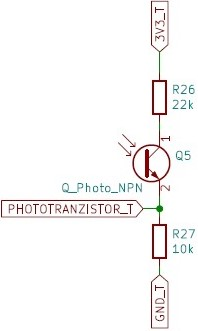
\includegraphics[scale=0.7]{obrazky/fototranzistor.jpg}
  \end{center}
  \caption[Zapojení fototranzistoru]{Zapojení fototranzistoru.}
\end{figure}

Do finální verze byl také přidán fototranzistor, který bude následně využíván pro automatickou regulaci jasu programovatelných LED typu WS2812C. Fototranzistor byl připojen na GPIO01 mikrokontroléru ESP32-C3. Na tomto 
pinu je k~dispozici AD převodník \cite{ESP_C3_dtsh}. Byl vybrán fototranzistor s~označením SMD3528C-50, který je citlivý na viditelné světlo \cite{Phototransistor}.
Tento fototranzistor byl umístěn také na vrchní DPS. 

Dále byl také 
přidán konektor pro připojení dalších programovatelných LED typu WS2812C, které mohou být na pásku připevněném po obvodu Univerzálního modulu. Tyto LED mohou zajišťovat, aby Univerzální modul mohl svítit 
nejen dopředu, ale i do stran. Tato funkcionalita opět rozšíří možnosti využití tohoto Univerzálního modulu. Na datový pin těchto programovatelných LED byl připojen do série ochranný rezistor R28 o~hodnotě 
180 $\Omega$, který 
zabraňuje zničení pinu mikrokontroléru EPS32-C3, kdyby byly omylem zkratován s~napájecím napětí. 

Bylo zapotřebí připojit k~mikrokontroléru i piny M0, M1 a AUX od LoRa modulu E22-900T22D. Na mikrokontroléru ale nebylo již dostatek volných pinů, a tak byl použit expander GPIO pinů. Vybraný expander
PCA9536D umožňuje připojení 4 GPIO a zároveň komunikuje s~mikrokontrolérem přes sběrnici $I^2C$ \cite{expander}. Kondenzátory C5 a C6, které byly připojeny k~expanderu slouží pro filtraci napájecího napětí. 
Kondenzátory mají hodnoty 10 $\mu$F a 100 nF. Pin AUX byl tedy připojen k~mikrokontroléru přímo přes GPIO5 a piny M0 a M1 byly připojeny k~GPIO0 
a~GPIO1 expanderu. Protože byly ještě volné GPIO piny na expanderu, bylo realizováno ještě samostatné vypínání napájení programovatelných LED, protože i když tyto LED nesvítí, tak mají stále spotřebu 
0,3 mA na jednu LED \cite{WS2812C_dtsh}. Při bateriově napájené aplikaci je to stále nemalý proud, a proto byl realizován právě tento samostatný vypínač napájení. 

\begin{figure}[!h]
  \begin{center}
    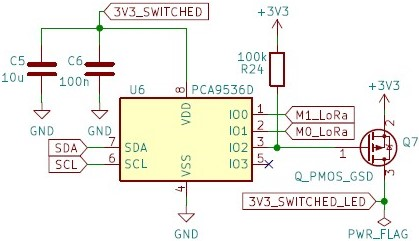
\includegraphics[scale=0.8]{obrazky/expander.jpg}
  \end{center}
  \caption[Zapojení expanderu]{Zapojení expanderu.}
\end{figure}

Ve finální verzi DPS byl použit posuvný vypínač se zahnutými vývody s~označením 1101M2S2AV2QE2 od firmy C\&K \cite{vypinac}.
Díky tomu mohl být vypínač umístěn na okraj DPS a nemusel být ručně pájen na drátkách. LED indikující přítomnost napájecího napětí 
3,3 V~a LED indikující nabíjení nebo plné nabití baterie byly dány na okraj spodní DPS tak, aby bylo možné je vidět, ale zároveň aby při používání Univerzálního modulu při hře nemohly zmást. LED indikující přítomnost 
napájecího napětí 5 V~byla odstraněna pro její nadbytečnost. 

Tranzistor PMOS, který slouží pro spínání napájecího napětí některým periferiím, byl přepojen z~pinu GPIO5 na pin GPIO2. Protože je pin GPIO2 konfiguračním pinem, tak byl přidán na gate tohoto tranzistoru pullup 
rezistor R25. Na pin GPIO5 byl připojen pin AUX od LoRa modulu E22-900T22D. Na pin GPIO0 byl připojen pin /CHANGE z~převodníku AT42QT1070 z~pinu GPIO3. Na pin GPIO3 byl připojen datový pin pro programovatelné LED, 
které budou připevněny na pásku po obvodu Univerzálního modulu. Zbytek periferií zůstal zapojený stejně. 

\begin{figure}[!h]
  \begin{center}
    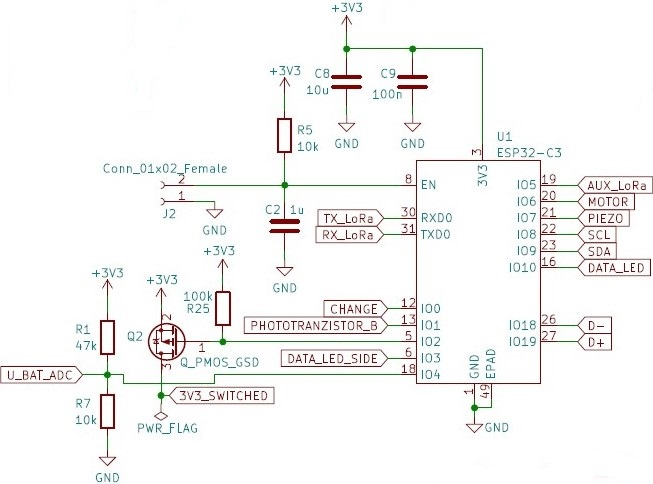
\includegraphics[scale=0.75]{obrazky/ESP32-C3_final.jpg}
  \end{center}
  \caption[Zapojení finální verze mikrokontroléru ESP32-C3]{Zapojení finální verze mikrokontroléru ESP32-C3.}
\end{figure}

K~napájecímu pinu VCC LoRa modulu byly připojeny kondenzátory C7 o~hodnotě 10 $\mu$F a C26 o~hodnotě 100 nF. Tyto kondenzátory slouží pro filtraci případných napěťových špiček. 

Byly přidány také zkratovací prokovy na EN pinu mikrokontroléru s~GND. Při zkratování je restartován mikrokontrolér. Tyto prokovy slouží pro snazší oživování a testování softwaru. Při provozu nebude propojka 
zkratována a bude zabráněno jejímu náhodnému zkratování. 

U~nabíjecího obvodu CN3058E byla zvětšena hodnota rezistoru R6 na 1 k$\Omega$, protože původní LED svítily až příliš. Naopak hodnota rezistoru R29 u~LED indikující napájecí napětíí byla zvětšena na 1 k$\Omega$, 
protože svit této LED nebyl téměř vidět. 

Rozložení součástek zvyšovače napětí bylo realizováno dle doporučení z~dokumentace. Prokovy k~signálu GND byly umístěny co nejblíže k~vstupnímu i výstupnímu kondenzátoru. Propojovací konektory byly 
umístěny po obvodu a byly na ně připojeny všechny potřebné signály. Napájecí napětí a GND signál byly přivedeny přes jeden konektor, aby se tak zlepšilo EMC. 

\begin{figure}[!h]
  \begin{center}
    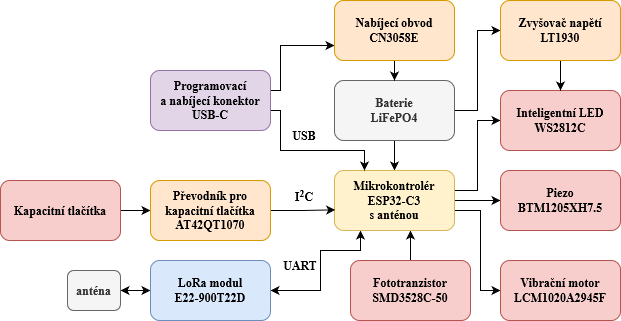
\includegraphics[scale=0.65]{obrazky/blokove_schema_finalni_verze.png}
  \end{center}
  \caption[Výsledné blokové schéma Univerzálního modulu]{Výsledné blokové schéma Univerzálního modulu.}
\end{figure}

Pouzdro na baterii bylo umístěno vertikálně do pravé části spodní DPS. Toto umístění bylo zvoleno kvůli možnosti připevnění Univerzálního modulu na dubové týblo. Týblo bude umístěno mezi spojenými DPS. 

Na DPS byly také umístěny 4 montážní otvory s průměrem 3 mm. Tyto otvory slouží pro sešroubování obou DPS dohromady pomocí distančních sloupků, aby byla zaručena pevnost. 

Při návrhu byly také brány v~potaz tekoucí proudy danými drahami. Tloušťky drah tomu byly přizpůsobeny a případné prokovy také. Například dráhy od baterie, jak k~nabíjecímu obvodu, tak k~USB mají tloušťku
2 mm, signálové dráhy mají tloušťku 0,125 mm a ostatní napájení dráhy mají tloušťku 1 mm. Prokovy mají vždy vrtanou díru stejně velkou, jako je tloušťka dráhy a okolní měď má průměr alespoň o~0,2 mm větší 
než vrtaná díra. U~dvounožičkových součástek byl také řešen thombstone efekt. Proto u~takových součástek byly dráhy vyvedeny stejně tlusté, případně alespoň co nejpodobnější. 
 
\newpage
\section{Výroba a oživení}

DPS byla následně opět vyrobena a osazena u~firmy JLCPCB. Opět nebyly k~dispoziciu firmy JLCPCB všechny potřebné součástky, takže některé byly osazeny ručně. Šlo o~kondenzátor C3 o~hodnotě 100 $\mu$F v~pouzdře 
0805, převodník pro kapacitní tlačítka AT42QT1070, piezo, posuvný vypínač, pouzdro na baterii a LoRa modul E22-900T22D. Obě DPS byly propojeny pomocí dlouhých pinheadů a dutinek. 
%napsat i oživení 

\begin{figure}[!h]
  \begin{center}
    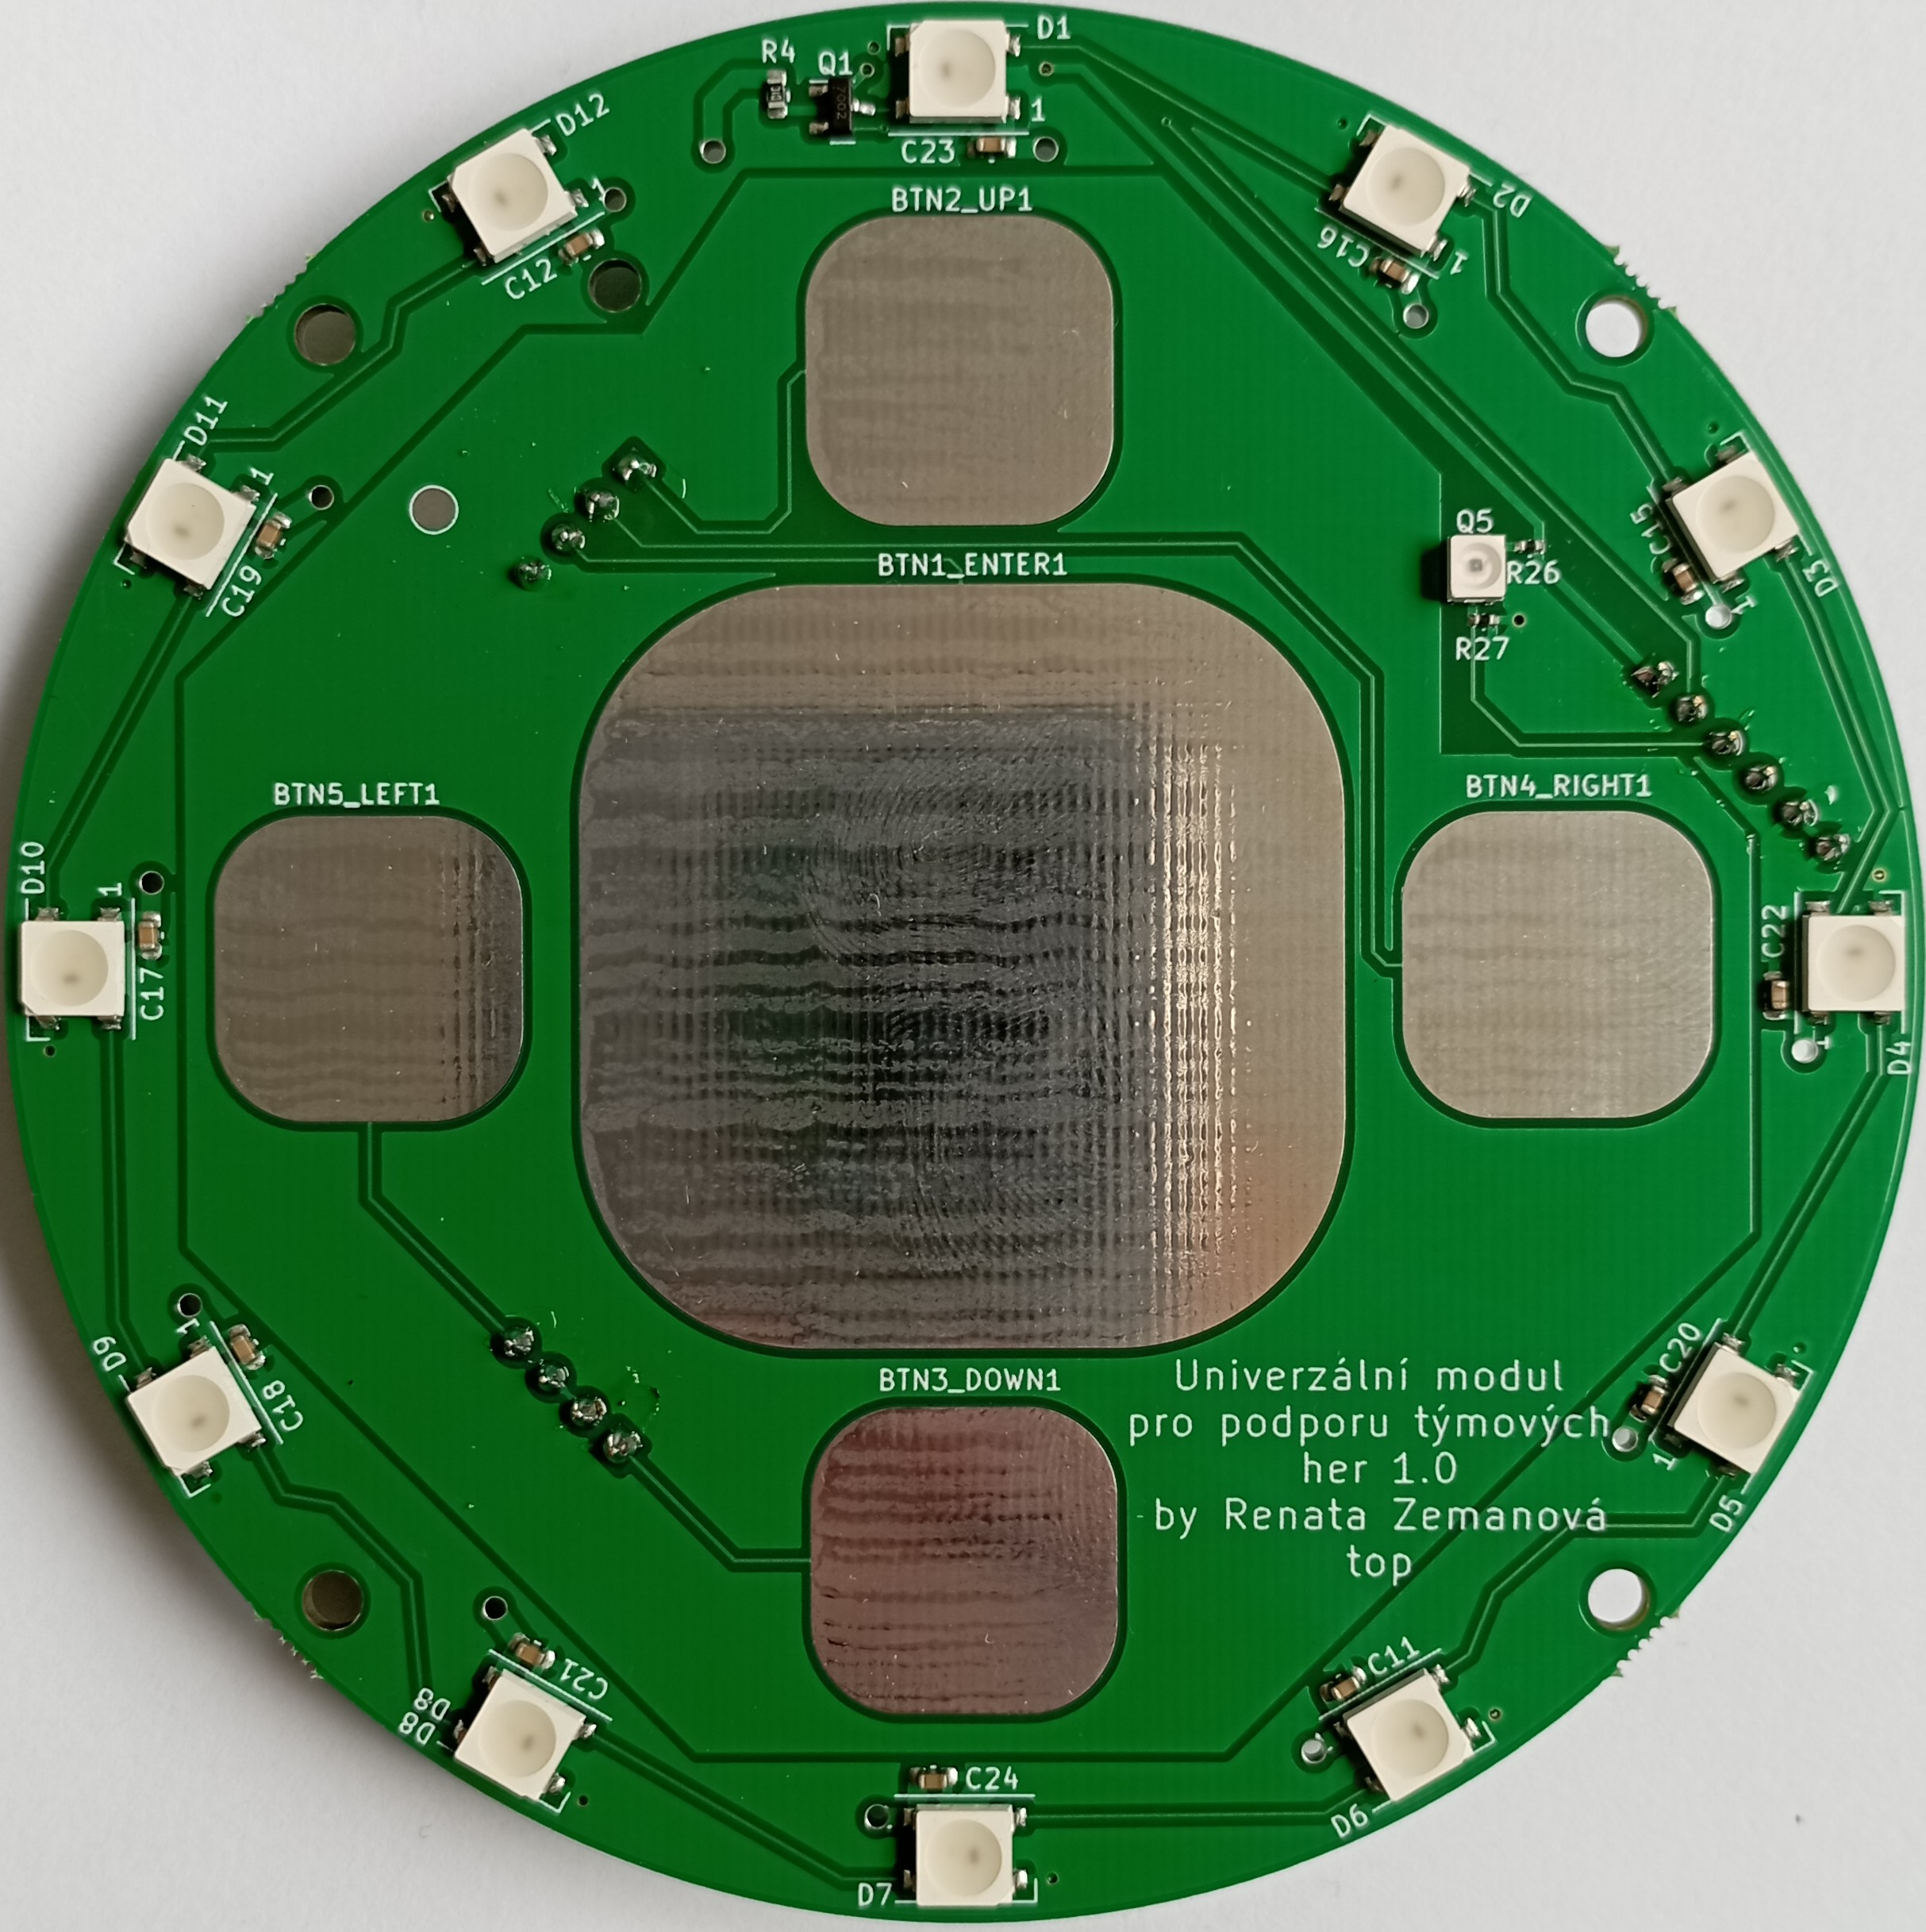
\includegraphics[scale=0.15]{obrazky/DPS_final_vrchni.jpg}
  \end{center}
  \caption[Výsledná DPS - vrchní část]{Výsledná DPS - vrchní část.}
\end{figure}

\begin{figure}[!h]
  \begin{center}
    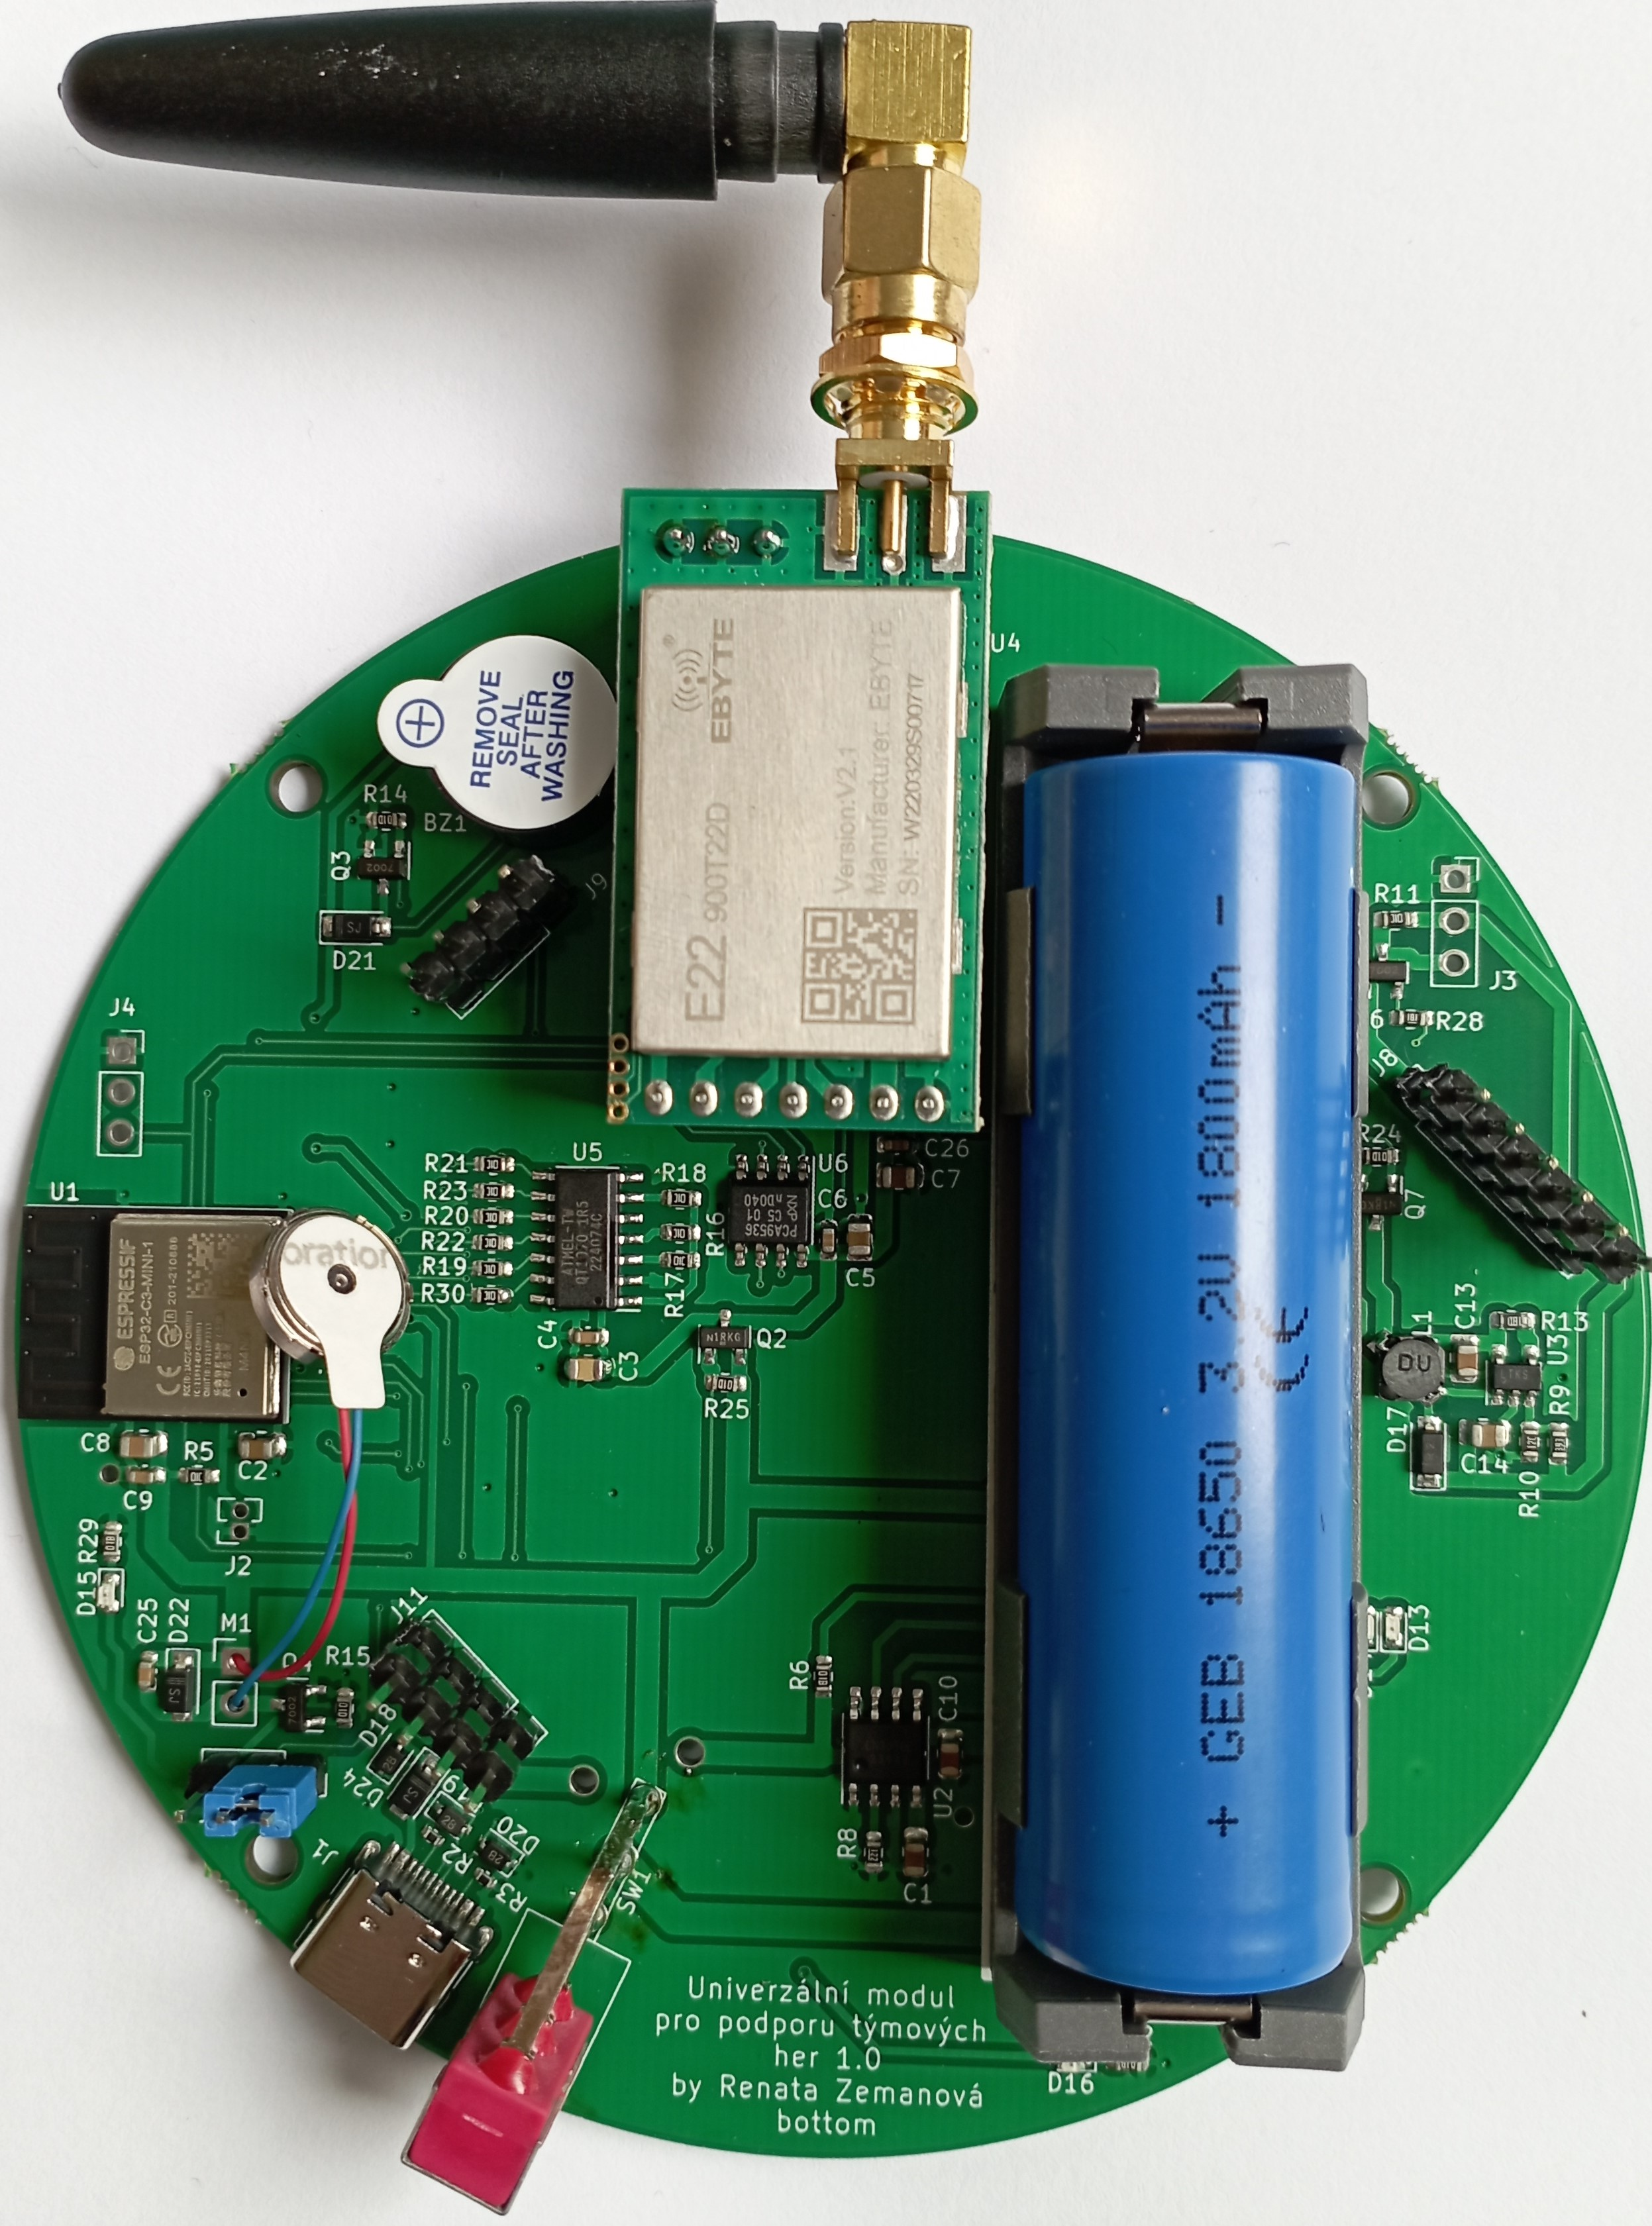
\includegraphics[scale=0.15]{obrazky/DPS_final_spodni.jpg}
  \end{center}
  \caption[Výsledná DPS - spodní část]{Výsledná DPS - spodní část.}
\end{figure}

\chapter{Firmware}
V~následující kapitole je popsán firmware Univerzálního modulu. Jsou zde popsány funkce, které byly vytvořeny pro následnou tvorbu softwaru Univerzálního modulu a~pro usnadnění práce s~ním. Univerzální 
modul je programován v~jazyce C++ a je využit Arduino framework, který mikrokontroléry typu ESP32 podporují.  

\section{Hlavní knihovna}
Hlavní knihovna sdružuje veškeré funkce, které jsou Univerzálnímu modulu k~dispozici. Tato knihovna obsahuje funkce pro práci s~kapacitními tlačítky, programovatelnými LED, WiFi, piezem, vibračním 
motorem i fototranzistorem. 

Pro práci s~programovatelnými LED byla využita knihovna Adafruit\_NeoPixel.h. V~hlavní knihovně byly vytvořeny funkce, které umožňují rozsvítit konkrétní barvou jednotlivé LED nebo všechny současně. Také 
je lze jednotlivě nebo všechny zhasnout. Byly vytvořeny také funkce pro blikání. 

Pro práci s~tlačítky byly implementovány funkce, které zjišťují, zda je některé z~tlačítek stisknuto. Každé tlačítko má svoji funkci. V~některých případech není zapotřebí vědět, které z~tlačítek je stisknuto, 
ale zda je vůbec některé z~nich stisknuto. Pro tyto účely vznikla funkce, která to umí zjistit. 

Dále byly vytvořeny funkce pro zapnutí a~vypnutí pieza a zároveň pro zapnutí a~vypnutí vibračního motoru. 

Byla vytvořena funkce pro vyčítání hodnot z~fototranzistoru. Tato funkce je zakomponováno ve funkci, která nastavuje jas programovatelných LED.

Pro hlídání stavu nabití baterií byly vytořeny funkce, které měří napětí na baterii a zjišťují, zda je baterie dostatečně nabitá, či nikoli. 

Dále knihovna obsahuje funkci pro vypnutí napájení periferiím, které jsou náročnější na spotřebu. Tato funkce existuje také pouze pro programovatelné LED. Tyto funkce mohou být využity právě při indikaci 
nízkého bateriového napětí.

Pro práci s~permanentní pamětí byly vytvořeny funkce, které umožňují z~permanentní paměti číst, nebo do ní zapisovat. 

\section{Práce s~kapacitními tlačítky}
Pro práci s~kapacitními tlačítky byla vytvořena speciální knihovna, protože existující knihovna AtTouch.h neposkytovala funkce, které jsou pro Univerzální modul zapotřebí. V~této knihovně se také 
vyskytují chyby, které vytvořená knihovna eliminuje.

Převodník AT42QT1070, který převádí signál z~kapacitních tlačítek, komunikuje po sběrnici $I^2C$. Proto byla využita knihovna Wire.h, která poskytuje funkce pro práci se sběrnicí $I^2C$.

Funkce knihovny pracují se vzorky naměřené kapacity z~kapacitních tlačítek. Tyto hodnoty jsou vyčítány z~registu Key Signal převodníku AT42QT1070 \cite{conv_cap_but_AT42QT1070_dtsh}. Poté jsou vyhodnoceny, zda je na 
tlačítku detekován stisk, či nikoli. Stisk je detekován rozdílem naměřené a referenční hodnoty. 

Pokud je detekován stisk, tak je ještě počkáno, zda stisk trvá. Tak je zabráněno falešným detekcím. Pokud stisk trvá, tak je signalizován stisk tlačítka. Pokud netrvá, tak je vyhodnocen jako falešný a naměřený vzorek 
není dále zpracováván.

Pokud není detekován stisk, tak je hodnota započítána do průměru předchozích hodnot kapacity tlačítka, když není stisknuto. Tento průměr je používán jako referenční hodnota pro detekci stisku tlačítka. Je to z~důvodu 
změny prostředí. Pokud se změní prostředí, ve kterém Univerzální modul pracuje, tak se změní i vlastní kapacita tlačítek. Prostředí se ale nikdy nemění skokově. Díky tomu se referenční hodnota přizpůsobuje pracovnímu 
prostředí a nedochází tak k~falešným detekcím stisku tlačítka. 

Funkce s~názvem tick proto musí být volána pravidelně, aby neustále docházelo k~obnově referenční hodnoty kapacity tlačítek. 

Knihovna také zajišťuje kalibraci tlačítek po startu Univerzálního modulu. Z~tohoto důvodu nesmí být při startu stisknuto žádné tlačítko. Hodnoty tlačítek z~kalibrace jsou počáteční hodnotou reference pro detekci stisku. 

Nad touto mechanikou pak existuje funkce, která přímo poskytuje informaci, zda je tlačítko stisknuto, či nikoli. 

\section{Vzdálená konfigurace}
Vzdálená konfigurace probíhá připojením telefonu přes WiFi k~Univerzálnímu modulu. Pro práci s~WiFi a serverem jsou použity knihovny WiFi.h, esp\_wifi.h, WiFiUdp.h a WebServer.h. 

Po stisku tlačítek nahoru a dolů současně je Univerzální modul přepnut do konfiguračního módu. Do tohoto módu lze přejít pouze po dobu 5 minut od zapnutí Univerzálního modulu, aby v~průběhu hry nemohl 
být omylem přepnut do konfiguračního módu hráčem. Tento mód je signalizován blikáním všech LED modrou barvou. Je vytvořena WiFi síť, ke které se lze připojit, a je zapnut server. Telefon nebo notebook je připojen 
k~Univerzálnímu modulu přes WiFi s~názvem UniverzalniModul. Heslo k~této WiFi je univerzalnimodul. Po připojení je zapotřebí zadat do internetového vyhledávače IP adresu Univerzálního modulu. Jeho IP adresa 
je 192.168.4.1. Po zadání této IP adresy je načtena konfigurační webová stránka. Tato webová stránka byla vytvořena v~HTML kódu. Na této stránce jsou jednotlivé již existující naprogramované módy, ve kterých umí 
Univerzální modul pracovat. Všechny módy jsou ve zkratce popsány. U~většiny módů jsou také boxy pro vyplnění vstupních parametrů daného módu. Uživatelem je tedy vybrán mód, ve kterém má Univerzální modul pracovat, 
jsou vyplněny vstupní parametry tohoto módu a poté je stisknuto tlačítko daného módu, které zapíná konkrétní mód. 

\begin{figure}[!h]
  \begin{center}
    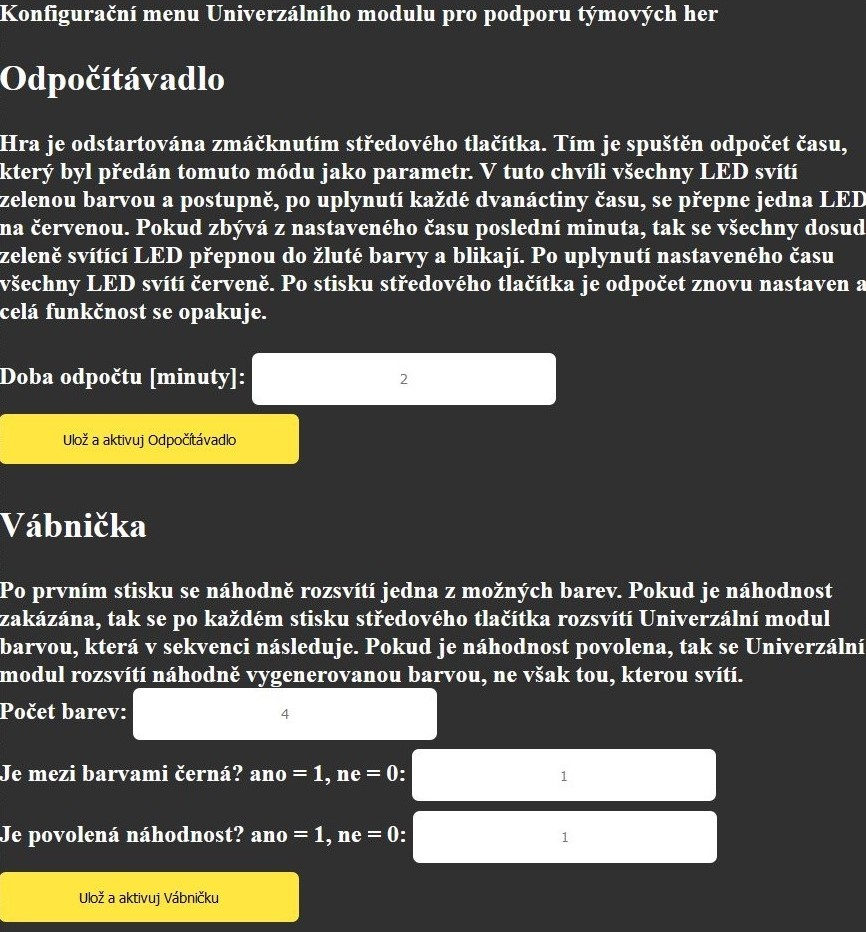
\includegraphics[scale=0.45]{obrazky/konfiguracni_webova_stranka.jpg}
  \end{center}
  \caption[Konfigurační webová stránka]{Konfigurační webová stránka.}
\end{figure}

Toto nastavení je uloženo do permamentní paměti mikrokontroléru. Pro práci s~permamentní pamětí je použita knihovna Preferences.h. Nastavení je také sdíleno ostatním Univerzálním modulům, které jsou v~té době zapnuty 
a neuběhlo u~nich 5 minut od jejich spuštění. Toto sdílení funguje tak, že nastavení je vysíláno přes WiFi na konrétním portu a může být zachyceno kýmkoli, kdo je připojen na tuto WiFi a kdo na tomto portu bude 
poslouchat. U~ostatních Univerzálních modulů je mód spuštěn automaticky hned po přijetí konfigurace. Tato konfigurace je také hned po přijetí uložena do permanentní paměti. Univerzální modul po restartování zapne 
nakonfigurovaný mód. Poté je WiFi i server vypnut. 

Po dobu 5 minut od startu Univerzálního modulu lze přijmout nastavení od jiného Univerzálního modulu. Univerzální modul poslouchá přes WiFi na daném portu. Pokud je nastavení sdíleno, tak je jiným Univerzálním modulem 
zachyceno a~staženo. Po stažení je toho nastavení uloženo do permamentní paměti a zároveň je konkrétní mód hned aktivován. 

\section{Celková funkce}
Univerzální modul po zapnutí nastaví všechna GPIO na vstupní nebo výstupní dle potřeby, případně zapne softwarové pullup rezistory. Poté je načtena konfigurace z~permamentní paměti. V~té je uložen poslední spuštěný 
mód  
i s~jeho konfigurací. Pokud je Univerzální modul spouštěn poprvé, tak je načten výchozí přednastavený mód s~nastavenými parametry. Zároveň je tato konfigurace uložena do permanentní paměti. Po dalším startu 
Univerzálního modulu pak bude z~permanentní paměti načítána poslední konfigurace. 

Poté je nastaven odpočet doby, po kterou může být přepnut Univerzální modul do konfiguračního módu. Tento čas je nastaven proto, aby se při hře nemohlo omylem stát, že by byl Univerzální modul přepnut do 
konfiguračního módu, protože do tohoto módu se přechází kombinací stisknutých tlačítek. 

Univerzální modul pak přechází do herního módu. V~herním módu je neustále spouštěn mód, který byl nastaven v~konfiguraci. Zároveň, pokud ještě nevypršel čas, do kdy je možné přejít do režimu konfigurace, tak 
je kontrolováno, zda není stisknuta kombinace tlačítek, kterou je zapnut konfigurační mód. V~každém cyklu je také čten stav tlačítek. Tato funkce je důležitá pro správné vyhodnocování stisku kapacitních tlačítek. 

\begin{figure}[!h]
  \begin{center}
    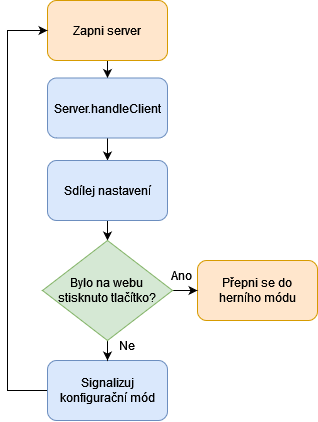
\includegraphics[scale=0.8]{obrazky/blokove_schema_modu_CONFIGURATION.png}
  \end{center}
  \caption[Blokové schéma konfiguračního módu]{Blokové schéma konfiguračního módu.}
\end{figure}

Pokud jsou na Univerzálním modulu stisknuta tlačítka nahoru a dolů současně, tak je Univerzální modul přepnut do konfiguračního módu. Tento mód je signalizován blikáním všech LED modrou barvou. V~tomto módu je zapnuta WiFi a server. Na 
tuto WiFi se lze připojit telefonem nebo notebookem. Po připojení k~WiFi a napsání IP adresy Univerzálního modulu do internetového vyhledávače je načtena webová stránka s~konfiguračním menu Univerzálního modulu. Po nastavení parametrů 
dané hry a stisku 
tlačítka pro spuštění dnaé hry je konfigurace sdílena pomocí WiFi. Konfigurace je tak k~dispozici ke stažení pro další Univerzální moduly, které jsou v~blízkosti konfigurovaného Univerzálního modulu a neuběhl u~nich daný čas od jejich 
startu. Po restartu Univerzální modul přechází zpět do herního módu. Je spuštěn mód, který byl nakonfigurován. Konfigurace této hry je uložena do permanentní paměti.


Pokud je dostupná WiFi jiného Univerzálního modulu, tak je Univerzální modul připojen na tuto WiFi a snaží se z~ní stáhnout novou konfiguraci. Pokud se podaří konfiguraci stáhnout, tak je zapnuta hra s~konfigurací,
která byla stažena z~WiFi jiného Univerzálního modulu. Konfigurace této hry je uložena do permanentní paměti. Stažení nové konfigurace je signalizováno půlvteřinovým probliknutím všech LED modrou barvou. 

Přepnutí do konfiguračního módu nebo stažení konfigurace z~jiného Univerzálního modulu je možné pouze 5 minut po zapnutí. 

\begin{figure}[!h]
  \begin{center}
    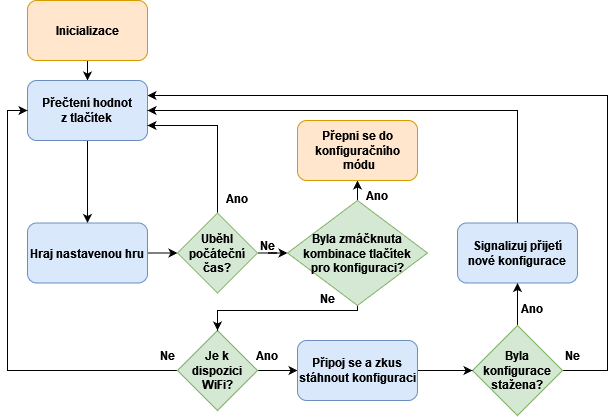
\includegraphics[scale=0.65]{obrazky/blokove_schema_modu_PLAY.png}
  \end{center}
  \caption[Blokové schéma herního módu]{Blokové schéma herního módu.}
\end{figure}

\chapter{Módy a využití}
V~této kapitole jsou popsány jednotlivé módy, které byly pro Univerzální modul vyvinuty, jako příklad využití tohoto zařízení. Všechny parametry, které dané módy přebírají, jsou zadávány 
v~rámci nastavení na konfigurační webové stránce.

\section{Klasický semafor}
Tento herní mód přebírá jako parametry minimální a maximální čas změny barvy svícení. 

Na začátku hry se s~pravděpodobností 0,5 rozsvítí všechny LED zelenou nebo červenou barvou. Následně je nastaven odpočet času, který je náhodný v~rozmezí minimálního a maximálního času změny. 
Po uplynutí tohoto času svítí na polovině LED žlutá barva. Na druhé polovině zůstává původní barva. Tento stav trvá 2 sekund. Následně se všechny LED přepnout do opačné barvy než byla původní. 
Pokud tedy v~prvním stavu svítily všechny LED červeně, tak nyní budou svítit zeleně a naopak. Tento stav bude opět aktivní po náhodně dlouhou dobu v~rozmezí minimálního a~maximálního času. Poté 
opět následuje stav, kdy jedna polovina LED zůstává stejná a druhá svítí žlutou barvou. Tento stav opět trvá 2 sekundy. Tato funkce se neustále opakuje. 

\begin{figure}[!h]
  \begin{center}
    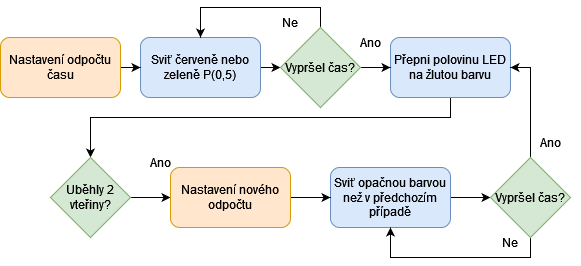
\includegraphics[scale=0.7]{obrazky/Klasicky_semafor_diagram.png}
  \end{center}
  \caption[Blokové schéma herního módu Klasický semafor]{Blokové schéma herního módu Klasický semafor.}
\end{figure}

Tento mód nahrazuje instruktora při omezování aktivit účastníků v~různých herních prvcích. Může sloužit jako omezovač přístupu k~surovinám ve strategických hrách, jako brána města, která se zavírá 
a otvírá a zamezuje nebo povoluje přístup k~tržišti. Osvědčuje se jako faktor náhody při časově omezených úkolech, například oběh hřiště. V~tomto módu mohou také Univerzální moduly náhodně řídit 
přístup do tzv. domečků - bezpečných zón, kde se lze ukrýt před útoky ostatních týmů v~bojových hrách.

\section{Odpočítávání}
Tento herní mód přebírá jako parametr čas k~odpočtu.

Hra je odstartována zmáčknutím středového tlačítka. Tím je spuštěn odpočet času, který byl předán tomuto módu jako parametr. V~tuto chvíli všechny LED svítí zelenou barvou a postupně, po uplynutí každé 
dvanáctiny času, se přepne jedna LED na červenou. Pokud zbývá z~nastaveného času poslední minuta, tak se všechny dosud zeleně svítící LED přepnou do žluté barvy a blikají. Po uplynutí nastaveného času 
všechny LED svítí červeně. Po stisku středového tlačítka je odpočet znovu nastaven a celá funkčnost se opakuje.  

\begin{figure}[!h]
  \begin{center}
    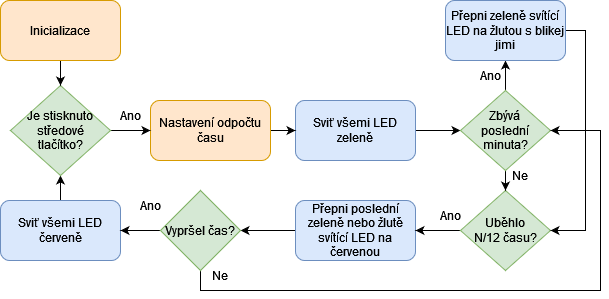
\includegraphics[scale=0.65]{obrazky/Odpocitavani_diagram.png}
  \end{center}
  \caption[Blokové schéma herního módu Odpočítávání]{Blokové schéma herního módu Odpočítávání.}
\end{figure}

Univerzální modul v~tomto módu může plně nahrazovat instruktora, který hlídá penalizaci hráčů, kteří mají strávit trestný čas mimo hru. Po spuštění se jim odpočítává penalizace, aniž by na místě musel 
někdo nastavovat stopky. Toto je velmi důležitou součástí výchovy k~fair-play. Univerzální modul může omezovat využitelnost herního místa nebo prvku. Například představovat odpočet do zasypání chodby, 
exploze výbušniny, nebo odjezdu vlaku. Opět platí, že se snižuje náročnost na instruktory, protože se herní místa mohou zavírat bez jejich přičinění, paralelně, nebo ve velkých vzdálenostech od sebe. 
Ve strategické hře tak například mohou simulovat postupné zavírání zdrojů surovin a přesouvat tak hru v~herním prostoru.

\section{Vábnička}
Tento herní mód přebírá jako parametr počet možných barev svícení, zda má mezi barvami být černá a zda má být posloupnost barev náhodná či nikoli.

Po prvním stisku se náhodně rozsvítí jedna z~možných barev. Pokud je náhodnost zakázána, tak se po každém stisku středového tlačítka rozsvítí Univerzální modul barvou, která v~sekvenci následuje. Pokud 
je náhodnost povolena, tak se Univerzální modul rozsvítí náhodně vygenerovanou barvou, ne však tou, kterou svítí. 

\begin{figure}[!h]
  \begin{center}
    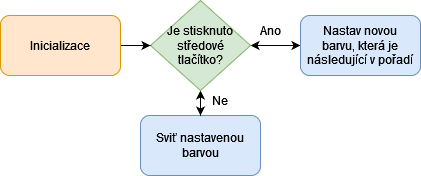
\includegraphics[scale=0.75]{obrazky/Vabnicka_diagram.png}
  \end{center}
  \caption[Blokové schéma herního módu Vábnička se zakázáním náhodnosti]{Blokové schéma herního módu Vábnička se zakázáním náhodnosti.}
\end{figure}

Univerzální modul v~tomto módu může sloužit jako vizuálně atraktivní, nebo v~noci použitelná, hrací kostka. V~náhodném střídání barev může fungovat jako omezovač průběhu herním prostorem s~podmínkou 
vlastnění klíče ve stejné barvě. V~přesném střídání barev může fungovat jako stopa posledního hráče. Hráč přepne Univerzální modul na svou barvu a dává tak na vědomí, že nikdo z~jeho týmu nemůže na 
stejné herní lokaci provádět herní úkony, dokud některý z~jiných týmů Univerzální modul nepřepne. Pro účely nočních her to řeší omezující pravidlo - na stejném stanovišti nesmí herní mechaniku použít 
stejný tým dvakrát za sebou. Odsud jméno módu - vábí k~truhle s~pokladem všechny, krom vysvíceného týmu.

\chapter{Voděodolnost}
Pro zajištění voděodolnosti byl zvolen obal z~průhledného silikonu. Do silikonu je DPS zalita, proto musela být navržena forma pro následné odlití. V~následující části je popsán postup 
návrhu formy a následná výroba silikonového pouzdra. Nejdříve byl celý proces otestován na prototypových DPS. Po odladění bylo vše překresleno podle finální verze DPS a byly zapouzdřeny
i finální verze Univerzálního modulu.  

\section{Prototyp}
Nejprve byl vyexportován z~programu KiCad 3D model celé DPS včetně všech součástek, které měly 3D model již z~interní knihovny. Pro součástky, které neměly 3D model a zároveň byly důležité 
pro výsledný vzhled pouzdra, byly 3D modely dokresleny v~programu SolidWorks. Pouzdra byla kreslena bez větších detailů. S~přesností byla kreslena pouze kritická místa, kde součástka ovlivňuje 
rozměry pouzdra nebo kde musí procházet pouzdrem až na povrch.
  
\begin{figure}[!h]
  \begin{center}
    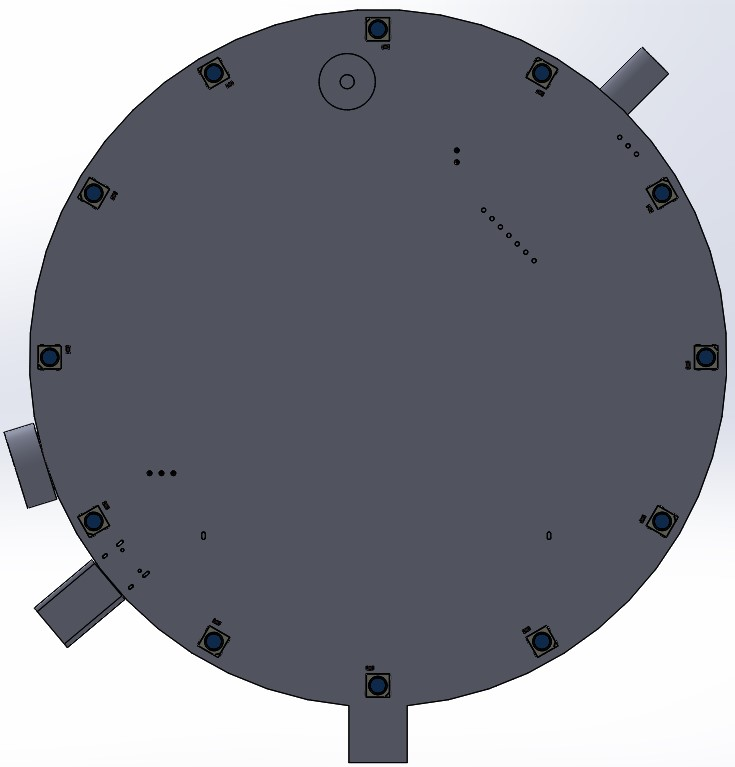
\includegraphics[scale=0.4]{obrazky/3D_model_predni.jpg}
  \end{center}
  \caption[3D model přední části DPS]{3D model přední části DPS.}
\end{figure}

Následně byl nakreslen model pouzdra, jak by mělo vypadat bez vložené DPS. Poté byla vytvořena sestava, kde byla DPS již vložené v~pouzdře. Z~pouzdra musely vyčnívat součásti, které nesmí být 
zality v~silikonu. Nesmí být zalit USB konektor, prostřednictvím něhož je Univerzální modul napájen a programován, dále vypínač a~piezo, protože by jinak nemohlo vydávat zvuk. 

Z~takto vytvořeného modelu byla vytvořena forma. Byl nakreslen válec, který byl z~každé strany o~3 mm větší než DPS s~obalem. Poté byl použit nástroj Kombinovat, který umožnil odečtení vytvořeného 
modelu DPS s~obalem, takže vznikla dutá forma pro potřebný tvar. Následně byla forma rozdělena na 2 díly, které na sebe pasují a~protínají v~polovině všechny otvory tak, aby se do těchto půlek 
dala DPS zavřít.

\begin{figure}[!h]
  \begin{center}
    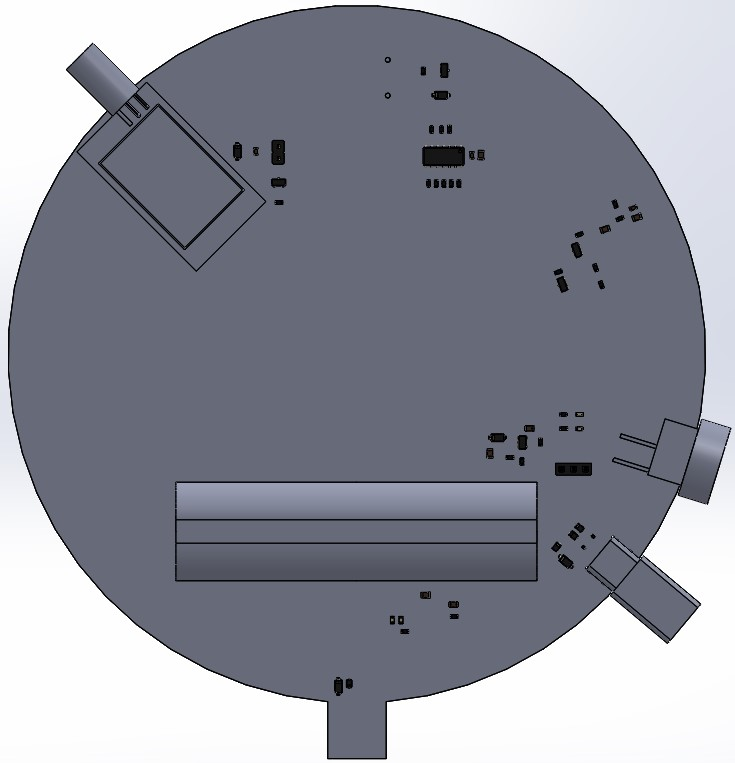
\includegraphics[scale=0.4]{obrazky/3D_model_zadni.jpg}
  \end{center}
  \caption[3D model zadní části DPS]{3D model zadní části DPS.}
\end{figure}

V~předním dílu formy byl ve spodní části vytvořen otvor o~průměru 2 mm pro vstřik silikonu. Ve spodní části byl proto, aby hladina silikonu postupně stoupala a~nevznikaly tak při vstřiku vzduchové 
kapsy a obal byl jednolitý. Do obou dílů formy byly vytvořeny také odvzdušňovací otvory. Tyto otvory mají průměr 0,5 mm a jsou rozmístěny po cca 2 cm, aby byl zajištěn odvod vzduchu a nevznikaly tak 
v~obalu vzduchové kapsy a silikon se dostal do všech potřebných míst. 

Protože silikon při tuhnutí zmenšuje svůj objem, musela být vytvořena zásobárna na silikon, který samospádem bude v~průběhu tuhnutí vtékat do formy. V~horní části byl tedy vytvořen zásobník, do kterého 
se při vstřikování silikonu po naplnění formy dostane silikon. Při procesu tuhnutí pak může silikon ze zásobníku přitékat do formy díky gravitaci. 

Forma na silikonový obal byla vytištěna na FMD 3D tiskárně. Nemohla být použita 3D tiskárna typu SLA, protože resin, ze kterého se v~SLA tiskárnách tiskne, zabraňuje tuhnutí použitého typu silikonu. 

Před zalitím Univerzálního modulu do formy byly pomocí vteřinového lepidla zalepeny boční otvory v~konektoru USB-C, aby silikon nevtekl těmito otvory dovnitř a neucpal tak tento konektor. DPS byla 
vložena do formy, utěsněna tavným lepidlem a stlačena pomocí svorek.

\begin{figure}[!h]
  \begin{center}
    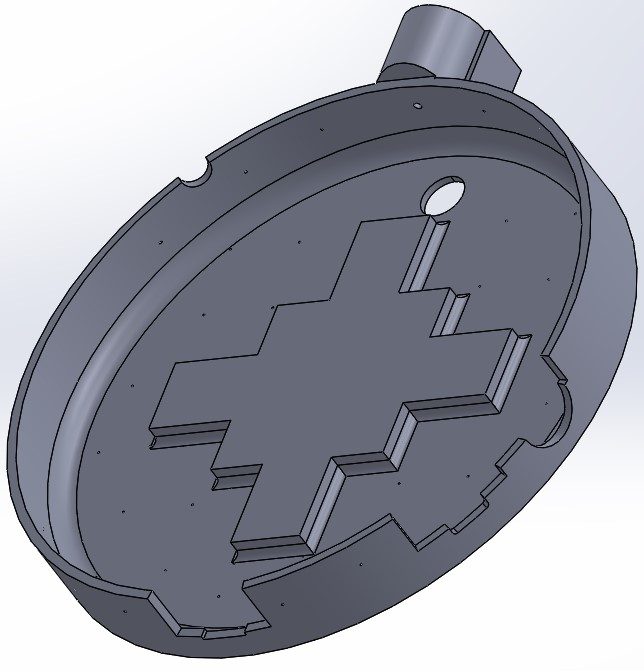
\includegraphics[scale=0.4]{obrazky/forma_predni.jpg}
  \end{center}
  \caption[3D model přední části formy]{3D model přední části formy.}
\end{figure}

Byl použit dvousložkový průhledný silikon GMS A30, který se míchá v~poměru 1:1 \cite{silikon}. Pomocí stříkačky byl silikon vtlačen do formy. Díky tomu, že otvor byl ve spodní části formy a zásobník 
nahoře, tak hladina postupně stoupala a nemohlo tak dojít ke vzniku vzduchových kapes. Až byl naplněn i vrchní zásobník, tak byl nátlakový otvor ucpán, aby silikon nevytekl. Tuhnutí tohoto silikonu 
při pokojové teplotě trvalo asi 5 hodin \cite{silikon}. Tuhnutí silikonu vyvolává exotermní reakci a zmenšuje se tak jeho objem. Proto byl postupně to vrchního zásobníku přidávám silikon, aby byl 
Univerzální modul zalit celý. 

\begin{figure}[!h]
  \begin{center}
    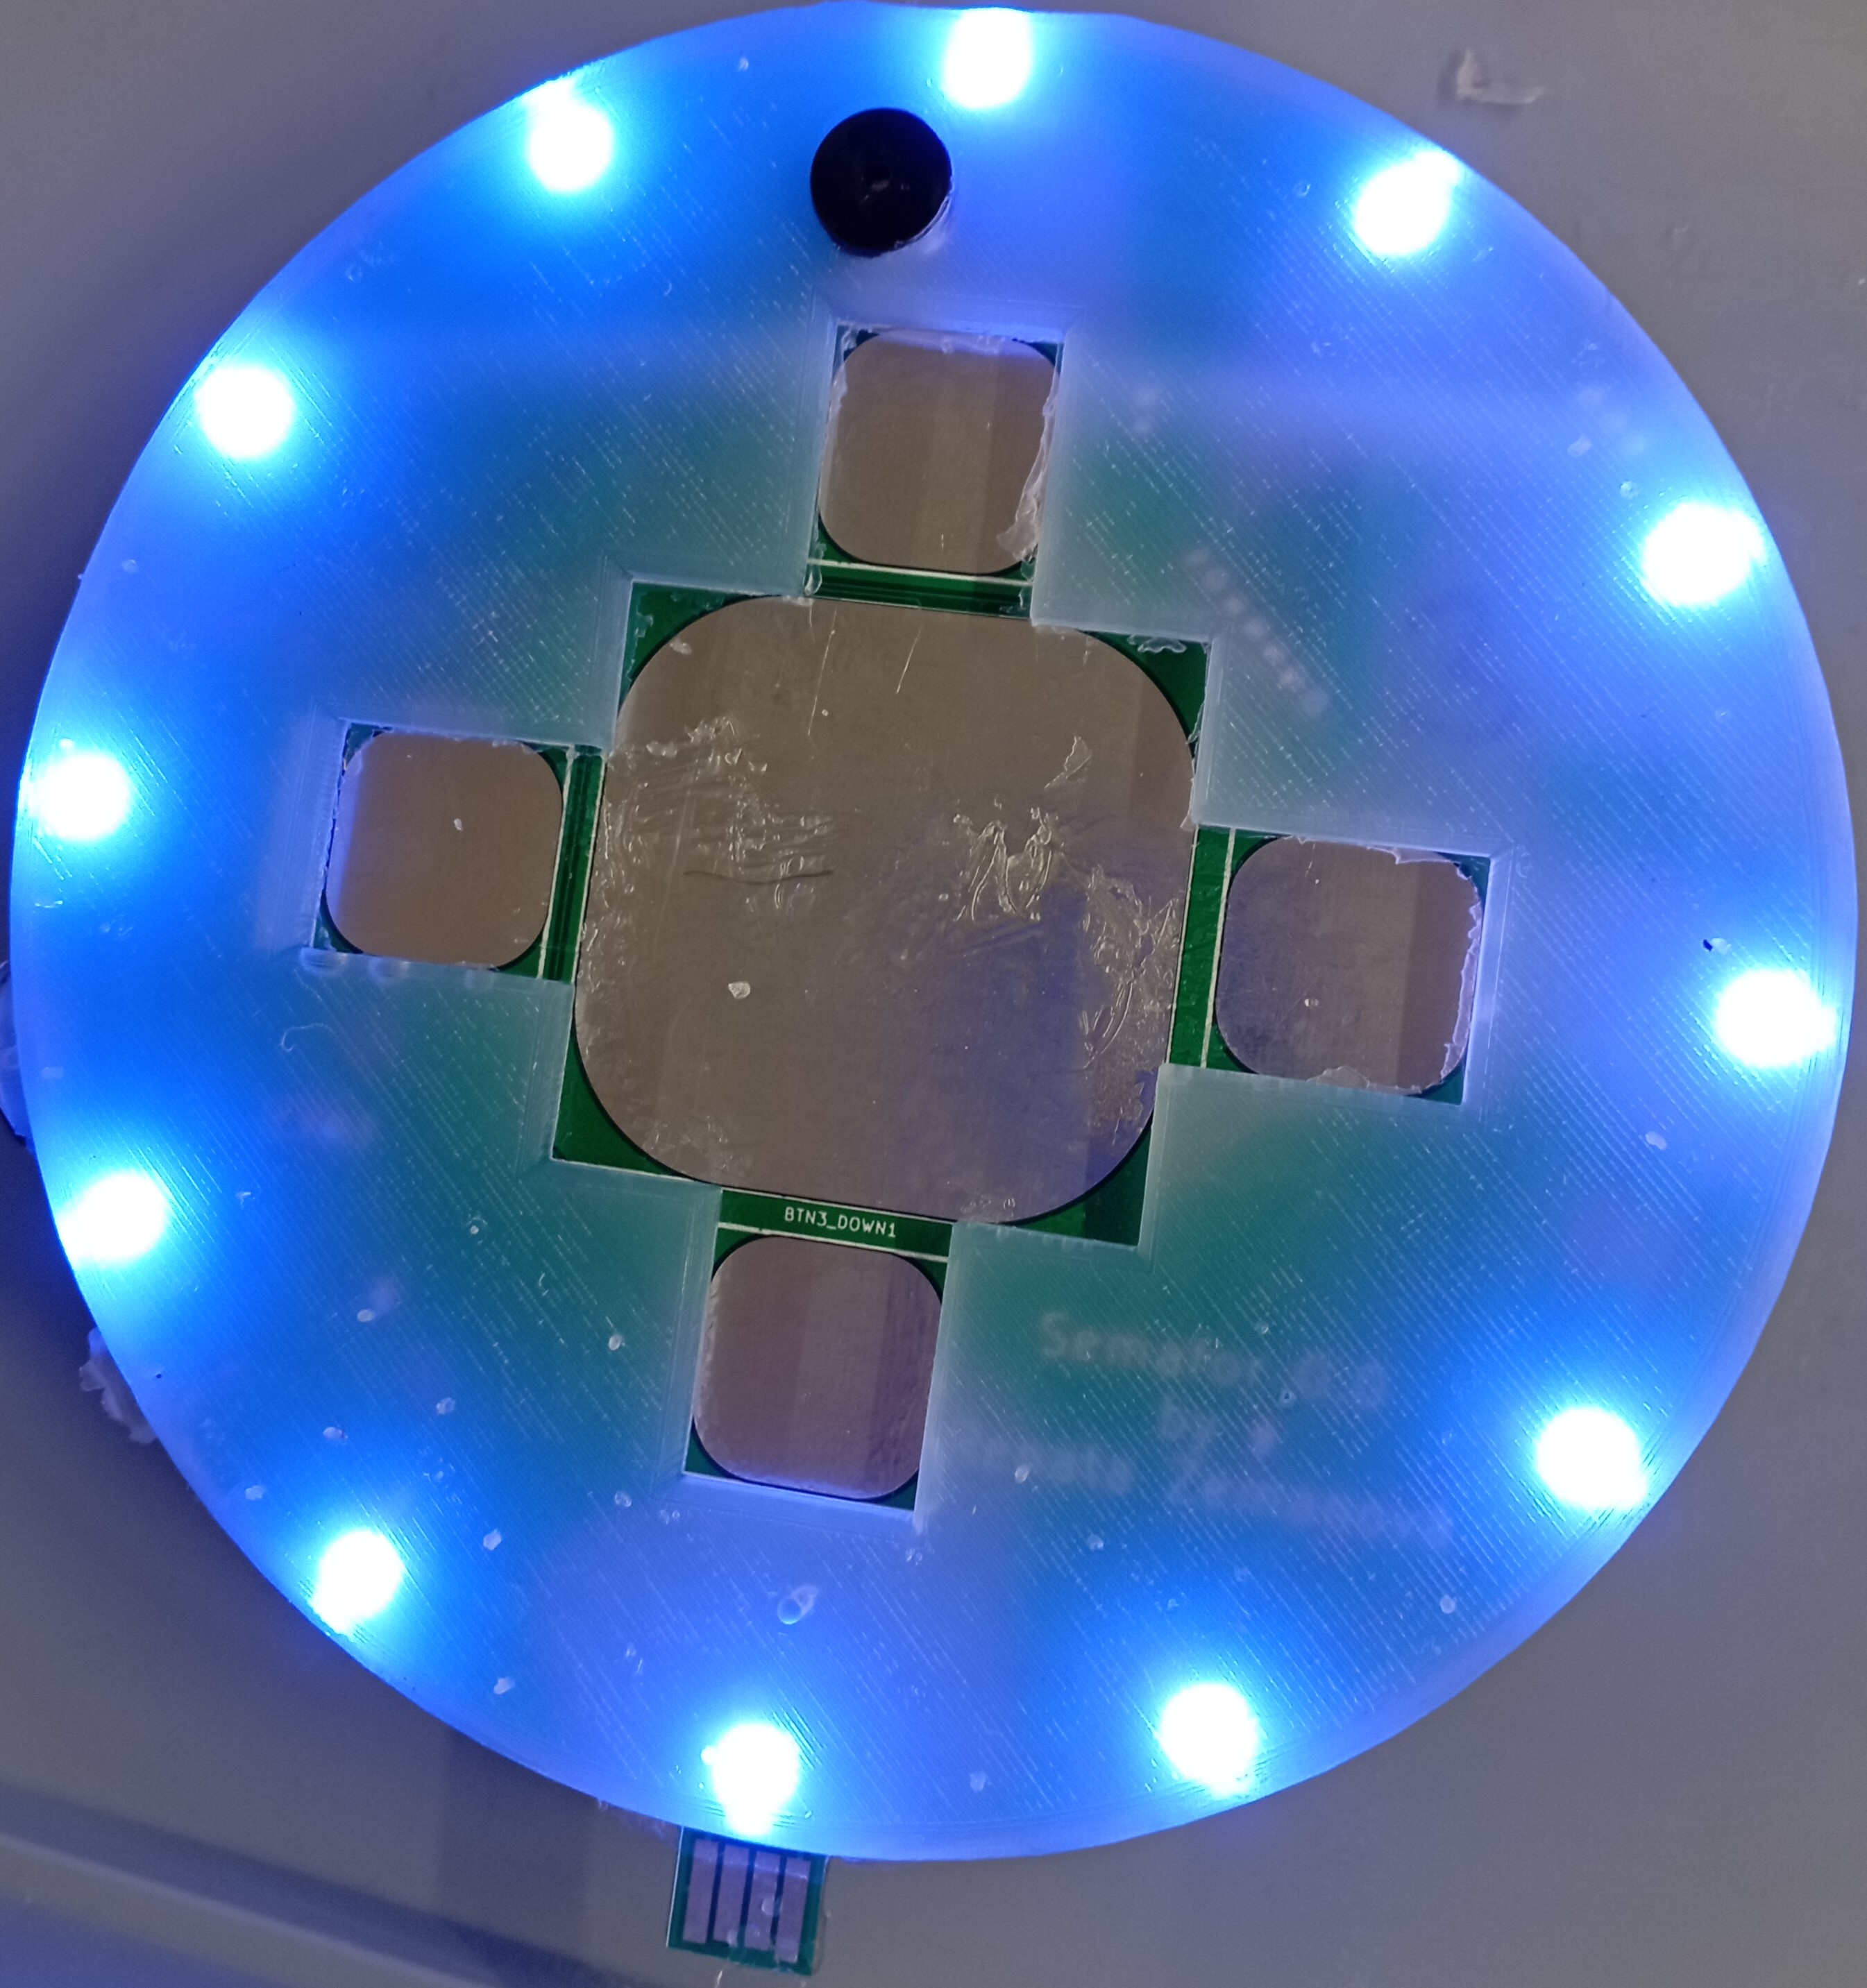
\includegraphics[scale=0.12]{obrazky/DPS_prototyp_v_silikonu.jpg}
  \end{center}
  \caption[Prototyp univerzálního modulu v~silikonu]{Prototyp univerzálního modulu v~silikonu.}
\end{figure}

Silikon špatně tuhnul a tvořily se v~něm vzduchové kapsy. Tenké vrstvy přes kapacitní tlačítka téměř neztuhly a v~některých místech se potrhaly. Zároveň spotřeba silikonu pro tak velký projekt byla velká. 
Na prototyp padlo více než 0,5 litru silikonu. Pro finální verzi by se musel postup opakovat a všechno části 3D modelu DPS musí být pečlivě s~velkou přesností vymodelovány. Ani tak není zaručena těsnost,
a proto se musí dotěsňovat například tavným lepidlem. Tento způsob výroby je velmi náročný a zdlouhavý. V~místech, kde není silikon spojen, tak navíc nedrží na DPS, protože silikon k~nničemnu nelepí, pouze 
sám k~sobě. 

\section{Finální verze}
Protože se silikonovým obalem u~prototypu byly problémy, tak byl obal finální verze Univerzálního modulu vytvořen jiným způsobem. Zároveň byl vybrán jednodušší postup a levnější řešení. 

Byla vymodelována kruhová krabička na finální verzi DPS, která pokrývá zadní a boční stranu Univerzálního modulu. V~bočních stranách jsou otvory pro nabíjecí konektor USB-C, vypínač, pásek programovatelných 
LED a pro anténu LoRa modulu. Univerzální modul také musí být nasazovatelný na dubové týblo o průměru 8 mm. Proto byl vytvořen otvor v krabičce a také byl vytištěn díl, který zabraňuje, aby týblo poškodilo 
elektroniku. Tento díl byl po vytištění vlepen do krabičky.  

Krabička byla vytištěna z PETG materiálu. Po vytištění byla DPS Univerzálního modulu sešroubována pomocí distančních sloupků o distanční délce 2 mm a šroubech M3 se zápustnou hlavou. Takto sešroubovaný Univerzální 
modul byl vložena do vytištěné krabičky. Ke krabičce byla DPS přilepena tavným lepidlem a~vrchní strana Univerzálního modulu byla zalakována čirým lakem. 

Toto řešení také zaručuje určitou možnou voděodolnost a je mnohem jednodušší na výrobu než v případě silikonové verze. 

%možná model

%fotka finální verze hotové i s obalem


